% =====================================================================
%  COS212 DFS Tutor -- Instructional Design Document
%  COS750 Educational Software Development, University of Pretoria
%  Compiles with pdfLaTeX, XeLaTeX, LuaLaTeX or Tectonic (Overleaf: pdfLaTeX)
% =====================================================================
\documentclass[11pt,a4paper]{article}

\usepackage{iftex}
\ifPDFTeX
  \usepackage[T1]{fontenc}
  \usepackage[utf8]{inputenc}
  \usepackage{lmodern}
  \usepackage[scaled=0.92]{helvet}
\else
  \usepackage{fontspec}
  \setsansfont{texgyreheros}[
    Extension=.otf, Scale=0.92,
    UprightFont=*-regular, BoldFont=*-bold,
    ItalicFont=*-italic, BoldItalicFont=*-bolditalic]
\fi

\usepackage[margin=2.3cm]{geometry}
\usepackage{microtype}
\usepackage{xcolor}
\usepackage{graphicx}
\usepackage{booktabs}
\usepackage{tabularx}
\usepackage{array}
\usepackage{longtable}
\usepackage{enumitem}
\usepackage{amsmath,amssymb}
\usepackage{float}
\usepackage{caption}
\usepackage{listings}
\usepackage{tikz}
\usetikzlibrary{arrows.meta,positioning,calc,fit,shapes.geometric,shapes.multipart,backgrounds}
\usepackage[hidelinks]{hyperref}

\setlength{\parskip}{0.45em}
\setlength{\parindent}{0pt}
\setlength{\emergencystretch}{2.5em}
\setlist{itemsep=0.15em, topsep=0.3em}
\captionsetup{font=small, labelfont=bf}
\renewcommand{\arraystretch}{1.25}
\newcolumntype{L}{>{\raggedright\arraybackslash}X}

% ---------------------------------------------------------------------
%  draw.io default palette
% ---------------------------------------------------------------------
\definecolor{dioBlueFill}{HTML}{DAE8FC}   \definecolor{dioBlueLine}{HTML}{6C8EBF}
\definecolor{dioGreenFill}{HTML}{D5E8D4}  \definecolor{dioGreenLine}{HTML}{82B366}
\definecolor{dioYellowFill}{HTML}{FFF2CC} \definecolor{dioYellowLine}{HTML}{D6B656}
\definecolor{dioOrangeFill}{HTML}{FFE6CC} \definecolor{dioOrangeLine}{HTML}{D79B00}
\definecolor{dioRedFill}{HTML}{F8CECC}    \definecolor{dioRedLine}{HTML}{B85450}
\definecolor{dioPurpleFill}{HTML}{E1D5E7} \definecolor{dioPurpleLine}{HTML}{9673A6}
\definecolor{dioGreyFill}{HTML}{F5F5F5}   \definecolor{dioGreyLine}{HTML}{666666}
\definecolor{edge}{HTML}{333333}

\tikzset{
  dio/.style={font=\sffamily\small, line width=0.75pt, >={Stealth[length=2.6mm,width=2mm,inset=0.7mm]}},
  box/.style={draw=dioBlueLine, fill=dioBlueFill, rounded corners=2.5pt, align=center,
              minimum height=9mm, minimum width=28mm, inner sep=1.5mm, font=\sffamily\small},
  boxc/.style 2 args={box, draw=#1Line, fill=#1Fill, #2},
  arrow/.style={->, draw=edge, line width=0.75pt},
  dep/.style={->, draw=edge, line width=0.75pt, dashed, >={Straight Barb[length=2.4mm,width=2.4mm]}},
  ret/.style={->, draw=edge, line width=0.7pt, dashed, >={Straight Barb[length=2mm,width=2mm]}},
  lbl/.style={font=\sffamily\scriptsize, fill=white, inner sep=1pt},
  note/.style={draw=dioYellowLine, fill=dioYellowFill, align=left, font=\sffamily\scriptsize,
               inner sep=2mm},
  treenode/.style={circle, draw=dioBlueLine, fill=dioBlueFill, minimum size=9.5mm,
                   inner sep=0pt, font=\sffamily\small\bfseries, line width=0.9pt},
  badge/.style={circle, draw=dioOrangeLine, fill=dioOrangeFill, minimum size=4.6mm,
                inner sep=0pt, font=\sffamily\scriptsize\bfseries, line width=0.6pt},
  usecase/.style={ellipse, draw=dioBlueLine, fill=dioBlueFill, minimum width=36mm,
                  minimum height=10mm, align=center, font=\sffamily\scriptsize, inner sep=0.5mm},
  umlclass/.style={rectangle split, rectangle split parts=3, draw=dioBlueLine,
                   rectangle split part fill={dioBlueFill,white,white},
                   rectangle split part align={center,left,left},
                   align=left, font=\sffamily\scriptsize, minimum width=46mm, inner sep=1.4mm},
  umlenum/.style={umlclass, rectangle split parts=2,
                  rectangle split part fill={dioPurpleFill,white}, draw=dioPurpleLine},
  stk/.style={draw=dioGreyLine, fill=dioGreyFill, minimum width=11mm, minimum height=6mm,
              font=\sffamily\small, inner sep=0pt},
  stktop/.style={stk, draw=dioOrangeLine, fill=dioOrangeFill, font=\sffamily\small\bfseries},
}

% Swimlane / container with a coloured title bar (draw.io "swimlane")
% #1 x-left, #2 y-top, #3 x-right, #4 y-bottom, #5 title, #6 colour prefix
\newcommand{\lane}[6]{%
  \draw[draw=#6Line, fill=white, line width=0.75pt] (#1,#2) rectangle (#3,#4);
  \draw[draw=#6Line, fill=#6Fill, line width=0.75pt] (#1,#2) rectangle (#3,{#2-0.62});
  \node[font=\sffamily\small\bfseries, anchor=west] at ({#1+0.25},{#2-0.31}) {#5};}

% UML stick-figure actor: #1 x, #2 y, #3 label, #4 coordinate name
\newcommand{\actor}[4]{%
  \begin{scope}[shift={(#1,#2)}, line width=0.8pt, draw=edge]
    \draw (0,0.62) circle (0.17);
    \draw (0,0.45) -- (0,-0.05);
    \draw (-0.3,0.28) -- (0.3,0.28);
    \draw (0,-0.05) -- (-0.24,-0.42);
    \draw (0,-0.05) -- (0.24,-0.42);
    \node[font=\sffamily\small] at (0,-0.68) {#3};
    \coordinate (#4) at (0,0.15);
  \end{scope}}

% UML 3-D deployment node: #1 x-left, #2 y-top, #3 x-right, #4 y-bottom, #5 title, #6 colour
\newcommand{\depnode}[6]{%
  \fill[#6Fill!70!#6Line] (#3,#2) -- ++(0.35,0.35) -- ({#3+0.35},{#4+0.35}) -- (#3,#4) -- cycle;
  \fill[#6Fill!85!#6Line] (#1,#2) -- ++(0.35,0.35) -- ({#3+0.35},{#2+0.35}) -- (#3,#2) -- cycle;
  \draw[draw=#6Line, line width=0.75pt] (#1,#2) -- ++(0.35,0.35) -- ({#3+0.35},{#2+0.35})
        -- ({#3+0.35},{#4+0.35}) -- (#3,#4);
  \draw[draw=#6Line, line width=0.75pt] (#3,#2) -- ++(0.35,0.35);
  \draw[draw=#6Line, fill=#6Fill, line width=0.75pt] (#1,#2) rectangle (#3,#4);
  \node[font=\sffamily\small, anchor=north, align=center] at ({(#1+#3)/2},{#2-0.12}) {#5};}

% ---------------------------------------------------------------------
%  Code listings
% ---------------------------------------------------------------------
\definecolor{codebg}{HTML}{F7F7F7}
\definecolor{codekw}{HTML}{1F4E94}
\definecolor{codecm}{HTML}{5A7F4B}
\definecolor{codestr}{HTML}{A0522D}
\lstdefinestyle{java}{
  language=Java, basicstyle=\ttfamily\footnotesize, keywordstyle=\color{codekw}\bfseries,
  commentstyle=\color{codecm}\itshape, stringstyle=\color{codestr},
  backgroundcolor=\color{codebg}, frame=single, rulecolor=\color{black!15},
  numbers=left, numberstyle=\tiny\color{black!45}, xleftmargin=1.6em, framexleftmargin=1.4em,
  showstringspaces=false, breaklines=true, tabsize=4, columns=fullflexible, keepspaces=true}
\lstdefinestyle{json}{
  basicstyle=\ttfamily\footnotesize, backgroundcolor=\color{codebg}, frame=single,
  rulecolor=\color{black!15}, showstringspaces=false, breaklines=true,
  stringstyle=\color{codestr}, morestring=[b]", columns=fullflexible, keepspaces=true}

\newcommand{\code}[1]{\texttt{#1}}

% =====================================================================
% ---------------------------------------------------------------------
%  Extra styles used only in the ID document
% ---------------------------------------------------------------------
\tikzset{
  tvisited/.style={treenode, draw=dioGreyLine, fill=dioGreyFill, text=dioGreyLine},
  tcurrent/.style={treenode, draw=dioOrangeLine, fill=dioOrangeFill, line width=1.8pt},
  tstack/.style={treenode, dashed, line width=1.1pt},
  tfound/.style={treenode, draw=dioGreenLine, fill=dioGreenFill, line width=1.4pt},
  wfbtn/.style={draw=dioGreyLine, fill=white, rounded corners=2pt, minimum height=6.5mm,
                inner xsep=2.5mm, font=\sffamily\scriptsize},
  wfbtnp/.style={wfbtn, draw=dioBlueLine, fill=dioBlueFill, font=\sffamily\scriptsize\bfseries},
  tick/.style={circle, fill=dioGreyLine, text=white, inner sep=0pt, minimum size=3.6mm,
               font=\sffamily\tiny\bfseries},
}

% Browser window frame for wireframes: #1 width, #2 height (negative y), #3 address
\newcommand{\browser}[3]{%
  \draw[draw=dioGreyLine, fill=white, line width=0.8pt, rounded corners=3pt] (0,0) rectangle (#1,-#2);
  \draw[draw=dioGreyLine, fill=dioGreyFill, line width=0.8pt, rounded corners=3pt]
       (0,0) -- (#1,0) -- (#1,-0.6) -- (0,-0.6) -- cycle;
  \foreach \c/\x in {dioRedLine/0.3, dioYellowLine/0.6, dioGreenLine/0.9}
    \fill[\c] (\x,-0.3) circle (0.09);
  \draw[draw=dioGreyLine, fill=white, rounded corners=4pt] (1.4,-0.15) rectangle ({#1-0.4},-0.45);
  \node[font=\sffamily\tiny, text=dioGreyLine, anchor=west] at (1.55,-0.3) {#3};}

% =====================================================================
\begin{document}

\begin{titlepage}
  \centering
  \vspace*{2.5cm}
  {\large University of Pretoria \textperiodcentered{} Department of Computer Science\par}
  \vspace{0.3cm}
  {\large COS750 Educational Software Development\par}
  \vspace{2.2cm}
  {\Huge\bfseries COS212 DFS Tutor\par}
  \vspace{0.5cm}
  {\Large Depth-First Search on a Binary Search Tree\par}
  \vspace{0.3cm}
  {\large Instructional Design Document (ID Document)\par}
  \vspace{2.5cm}
  \begin{tabular}{@{}ll@{}}
    \textbf{Version} & 1.0 \\
    \textbf{Date} & 28 October 2026 \\
    \textbf{Status} & Draft for team review \\
    \textbf{Companion document} & SE Document v1.1 (requirements and architecture) \\
    \textbf{Group} & \rule{6cm}{0.4pt} \\
  \end{tabular}
  \vfill
  {\small This document describes the educational design of the COS212 DFS Tutor: who it is for,
  what students should learn, how the content is structured and presented, how students are
  kept motivated, how their progress is assessed and supported, and how we will evaluate whether
  the app works. The use of generative AI is acknowledged in Appendix~\ref{app:genai}.\par}
\end{titlepage}

\tableofcontents
\newpage

% =====================================================================
\section{Introduction}
% =====================================================================

\subsection{Purpose of this document}

The COS212 lecturer wants students to arrive at the lecture on depth-first search having already
met the idea once, in a low-pressure setting, with something like a tutor beside them. Our answer
is the COS212 DFS Tutor: a short, self-paced web app that teaches depth-first search (DFS) on a
binary search tree (BST), lets students practise it, checks whether they are ready, and helps them
if they are not.

The SE document describes how the app is built. This document describes how it \emph{teaches}.
It sets out the instructional design approach we followed, the analysis behind our decisions, the
learning outcomes, the learning theories we drew on, how the app caters for different learners and
keeps them motivated, how assessment and scaffolding work, and how we plan to evaluate the result.
Section~\ref{sec:reflect} reflects honestly on the choices we made and their limits.

\subsection{The brief in one paragraph}

The examination specification asks for a prototype that teaches one core data structure and one
core algorithm from CS2023 \cite{cs2023} to students who \emph{have not yet seen them}. The app must
include some form of assessment that can be used to give students additional scaffolding before
the lecture. We chose the binary search tree and depth-first search. The full session is designed
to take about 20 to 25 minutes.

\subsection{How to read this document}

The document follows the five phases of our instructional design approach, ADDIE: Analysis
(Section~\ref{sec:analysis}), Design (Sections~\ref{sec:outcomes}--\ref{sec:assess}),
Development (Section~\ref{sec:dev}), Implementation (Section~\ref{sec:impl}) and Evaluation
(Section~\ref{sec:eval}). The complete learner-facing lesson text, the full quiz bank, a glossary
and our evaluation instruments are in the appendices, so that a reader can see exactly what a
student will see.

% =====================================================================
\section{Instructional design approach}
\label{sec:approach}
% =====================================================================

\subsection{Why ADDIE}

We use \textbf{ADDIE} (Analysis, Design, Development, Implementation, Evaluation)
\cite{branch2009} as our instructional design approach. We considered three alternatives:

\begin{itemize}
  \item \textbf{SAM} (Successive Approximation Model) suits teams that can run many quick
        prototype-and-test rounds with real learners. We have two weeks and limited access to
        students who have not done COS212 yet, so we cannot iterate that often.
  \item \textbf{Dick and Carey} is thorough but heavy for a short prototype; several of its ten
        steps (for example a full performance context analysis) would cost more time than they
        return here.
  \item \textbf{Merrill's First Principles} \cite{merrill2002} describe what good instruction
        contains rather than how to run a project. We use them as a check on our design
        (Section~\ref{sec:merrill}), not as the process.
\end{itemize}

ADDIE fits our situation best. It is easy for every group member to follow, it maps neatly onto
the two-week plan in the SE document, and it has a clear place for evaluation. We use it in its
modern, iterative form: evaluation is not a final step but runs alongside every phase, as
Figure~\ref{fig:addie} shows.

Inside the Design phase we need a way to sequence a single lesson. For that we use
\textbf{Gagné's Nine Events of Instruction} \cite{gagne2005}. ADDIE tells us how to run the project;
Gagné tells us what order the screens should come in. The two work at different levels and do not
compete.

\begin{figure}[H]
\centering
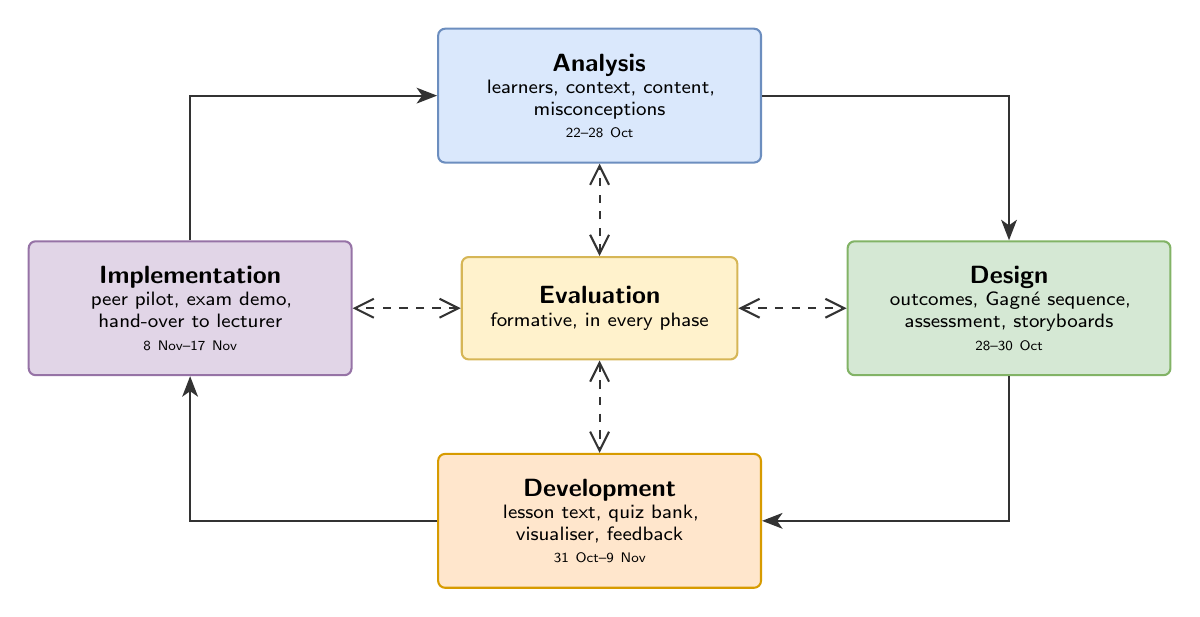
\begin{tikzpicture}[dio]
  \tikzset{ph/.style={boxc={#1}{minimum width=40mm, text width=38mm, minimum height=17mm,
                      font=\sffamily\scriptsize}}}
  \node[ph=dioBlue]   (a) at (0,2.7)   {\textbf{\small Analysis}\\ learners, context, content,\\ misconceptions\\ {\tiny 22--28 Oct}};
  \node[ph=dioGreen]  (d) at (5.2,0)   {\textbf{\small Design}\\ outcomes, Gagné sequence,\\ assessment, storyboards\\ {\tiny 28--30 Oct}};
  \node[ph=dioOrange] (v) at (0,-2.7)  {\textbf{\small Development}\\ lesson text, quiz bank,\\ visualiser, feedback\\ {\tiny 31 Oct--9 Nov}};
  \node[ph=dioPurple] (i) at (-5.2,0)  {\textbf{\small Implementation}\\ peer pilot, exam demo,\\ hand-over to lecturer\\ {\tiny 8 Nov--17 Nov}};
  \node[boxc={dioYellow}{minimum width=34mm, text width=32mm, minimum height=13mm, font=\sffamily\scriptsize}]
       (e) at (0,0) {\textbf{\small Evaluation}\\ formative, in every phase};
  \draw[arrow] (a.east) -| (d.north);
  \draw[arrow] (d.south) |- (v.east);
  \draw[arrow] (v.west) -| (i.south);
  \draw[arrow] (i.north) |- (a.west);
  \foreach \n in {a,d,v,i} \draw[dep, <->] (e) -- (\n);
\end{tikzpicture}
\caption{ADDIE as we apply it, with evaluation at the centre of every phase.}
\label{fig:addie}
\end{figure}

% =====================================================================
\section{Analysis}
\label{sec:analysis}
% =====================================================================

\subsection{Learner analysis}

Our learners are second-year Computer Science students registered for COS212 at the University of
Pretoria. What we can reasonably assume about them:

\begin{longtable}{@{}p{4.2cm} p{10.6cm}@{}}
  \toprule
  \textbf{Characteristic} & \textbf{What it means for the design} \\
  \midrule
  \endhead
  Completed first-year programming & They can read simple Java-like code and know what an
      \code{if} statement and a loop are. We may show code, but never rely on it. \\
  No prior knowledge of BSTs or DFS & The specification is explicit about this. Every term is
      introduced before it is used, and the warm-up check catches students who do not know what
      a tree or a stack is. \\
  Mixed confidence with recursion & Some students find recursion frightening. We teach DFS with an
      explicit stack first, and only show the recursive version as an optional extra. \\
  Busy, self-directed, time-poor & The session must be short (about 20--25 minutes), work in
      one sitting, and make progress visible so they know how much is left. \\
  Studying on their own laptops & Laptop browser is the target platform; phones are out of scope
      for the prototype. \\
  Diverse language backgrounds & Many students study in their second or third language. We use
      short sentences, everyday words and a glossary, and avoid idioms where possible. \\
  Varied access needs & Some students are colour-blind or use the keyboard more than the mouse.
      Colour is never the only signal and everything works from the keyboard. \\
  \bottomrule
\end{longtable}

Because the app is used \emph{before} the lecture, it carries no marks. Motivation therefore has to
come from the experience itself and from students seeing that it will make the lecture easier
(Section~\ref{sec:motivation}).

\subsection{Context analysis}

\begin{itemize}
  \item \textbf{When:} two or three days before the COS212 lecture on tree traversal.
  \item \textbf{Where:} at home, in a lab or in residence, on a laptop browser, alone.
  \item \textbf{How long:} one sitting of about 20--25 minutes; the student can stop at any point.
  \item \textbf{Support available:} none in the moment. The app has to do the tutor's job:
        explain, check, hint and encourage.
  \item \textbf{Stakes:} none. The quiz is for the student's own information. Nothing is recorded
        or sent to the lecturer in this prototype.
\end{itemize}

\subsection{Content analysis: a learning hierarchy}

Following Gagné's idea of a learning hierarchy, we broke the target skill (``trace a DFS on a BST'')
into the smaller skills it depends on. Figure~\ref{fig:hierarchy} shows the result. Anything below
the dashed line is assumed entry behaviour; everything above it is taught by the app. The
hierarchy directly determines the order of the lesson: we teach from the bottom up.

\begin{figure}[H]
\centering
\resizebox{\linewidth}{!}{%
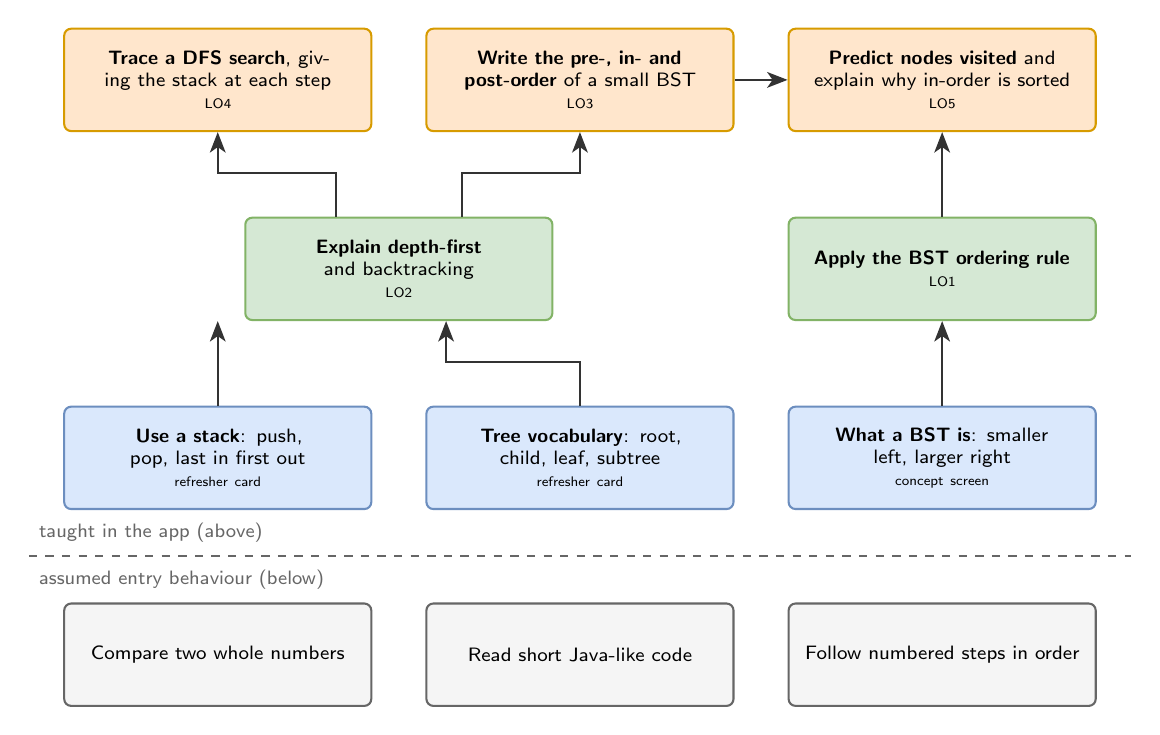
\begin{tikzpicture}[dio]
  \tikzset{hb/.style={boxc={#1}{minimum width=38mm, text width=36mm, minimum height=13mm,
                      font=\sffamily\scriptsize}}}
  \node[hb=dioOrange] (t1) at (-4.6,0) {\textbf{Trace a DFS search}, giving the stack at each step\\ {\tiny LO4}};
  \node[hb=dioOrange] (t2) at (0,0)    {\textbf{Write the pre-, in- and post-order} of a small BST\\ {\tiny LO3}};
  \node[hb=dioOrange] (t3) at (4.6,0)  {\textbf{Predict nodes visited} and explain why in-order is sorted\\ {\tiny LO5}};
  \node[hb=dioGreen]  (s1) at (-2.3,-2.4) {\textbf{Explain depth-first} and backtracking\\ {\tiny LO2}};
  \node[hb=dioGreen]  (s2) at (4.6,-2.4)  {\textbf{Apply the BST ordering rule}\\ {\tiny LO1}};
  \node[hb=dioBlue]   (p1) at (-4.6,-4.8) {\textbf{Use a stack}: push, pop, last in first out\\ {\tiny refresher card}};
  \node[hb=dioBlue]   (p2) at (0,-4.8)    {\textbf{Tree vocabulary}: root, child, leaf, subtree\\ {\tiny refresher card}};
  \node[hb=dioBlue]   (p3) at (4.6,-4.8)  {\textbf{What a BST is}: smaller left, larger right\\ {\tiny concept screen}};
  \draw[draw=dioGreyLine, dashed, line width=0.8pt] (-7,-6.05) -- (7,-6.05);
  \node[font=\sffamily\scriptsize, text=dioGreyLine, anchor=south west] at (-7,-6.0) {taught in the app (above)};
  \node[font=\sffamily\scriptsize, text=dioGreyLine, anchor=north west] at (-7,-6.1) {assumed entry behaviour (below)};
  \node[hb=dioGrey] (e1) at (-4.6,-7.3) {Compare two whole numbers};
  \node[hb=dioGrey] (e2) at (0,-7.3)    {Read short Java-like code};
  \node[hb=dioGrey] (e3) at (4.6,-7.3)  {Follow numbered steps in order};
  \draw[arrow] (p1.north) -- (p1.north |- s1.south) ;
  \draw[arrow] (p2.north) -- ++(0,0.55) -| ($(s1.south)+(0.6,0)$);
  \draw[arrow] (p3) -- (s2);
  \draw[arrow] ($(s1.north)+(-0.8,0)$) -- ++(0,0.55) -| (t1.south);
  \draw[arrow] ($(s1.north)+(0.8,0)$) -- ++(0,0.55) -| (t2.south);
  \draw[arrow] (s2) -- (t3);
  \draw[arrow] (t2) -- (t3);
\end{tikzpicture}}
\caption{Learning hierarchy for the session. Arrows point from a prerequisite to the skill that depends on it.}
\label{fig:hierarchy}
\end{figure}

\subsection{Misconception analysis}

Teaching works best when it is aimed at what students actually get wrong. From the literature on
algorithm visualisation and our own experience of learning this topic, we identified five likely
misconceptions. The COS212 tutor in our expert review (Section~\ref{sec:eval}) will be asked to
confirm or add to this list. Each one is targeted
at least three times in the app: once in the explanation, once in guided practice and once in the
quiz.

\begin{longtable}{@{}p{0.6cm} p{4.6cm} p{4.6cm} p{4.8cm}@{}}
  \toprule
  \textbf{ID} & \textbf{Misconception} & \textbf{What it looks like} & \textbf{How the app responds} \\
  \midrule
  \endhead
  M1 & Depth-first means level by level & After 50 the student picks 70, the other child of the
       root & Maze analogy; step player shows the walk going \emph{down}; quiz distractor with
       targeted feedback \\
  M2 & The stack is invisible or optional & Student cannot say what happens after a leaf &
       Stack panel is always visible; ``what is on top?'' is the first hint \\
  M3 & Pre-, in- and post-order are different walks & Student re-traces the tree from scratch for
       each order & ``Three orders, one walk'' screen; the code view shows only one line moving \\
  M4 & DFS uses the BST ordering to choose a direction & Student says DFS finds 80 in 3 steps &
       Explicit ``what DFS does \emph{not} do'' screen; comparison on the summary screen \\
  M5 & Pushing left first makes left come out first & Student writes the stack as [70, 30] after
       visiting 50 & Plate analogy (``last on, first off''); stack animation shows the order of pushes \\
  \bottomrule
\end{longtable}

\subsection{Needs summary}

Students need to (1) form a correct mental model of ``go deep, then back up'', (2) see the stack
that makes backtracking possible, (3) practise with feedback until the steps feel routine, and
(4) know honestly whether they are ready for the lecture. These four needs drive everything in
the Design phase.

% =====================================================================
\section{Learning outcomes and alignment}
\label{sec:outcomes}
% =====================================================================

\subsection{Learning outcomes}

Each outcome is written so that it can be observed and checked, and is tied to a level of the
revised Bloom's taxonomy \cite{anderson2001}. The audience for all outcomes is a COS212 student
working alone with the app.

\begin{longtable}{@{}p{0.9cm} p{2.0cm} p{12.0cm}@{}}
  \toprule
  \textbf{ID} & \textbf{Bloom level} & \textbf{By the end of the session, the student can\ldots} \\
  \midrule
  \endhead
  LO1 & Remember & state the BST ordering rule and name the data structure DFS uses to remember
        where to go back to (a stack), choosing correctly from four options. \\
  LO2 & Understand & explain in their own words what ``depth-first'' and ``backtracking'' mean,
        and identify the next node DFS visits from a given point in a tree. \\
  LO3 & Apply & write the pre-, in- and post-order of a BST with up to seven nodes, without
        errors. \\
  LO4 & Apply & trace a DFS search for a value on a BST with up to seven nodes, giving the stack
        contents after each step. \\
  LO5 & Analyse & predict how many nodes DFS visits for a given target, explain why it may visit
        more nodes than necessary, and explain why the in-order of a BST is always sorted. \\
  \bottomrule
\end{longtable}

We deliberately stop at \emph{Analyse}. Evaluating DFS against other search strategies is the job
of the lecture. The app ends by handing that question over (Section~\ref{sec:lesson}).

\subsection{Constructive alignment}

Biggs' principle of constructive alignment \cite{biggs1996} says that outcomes, learning activities
and assessment should all point at the same thing. Table~\ref{tab:align} shows how each outcome is
taught, practised and assessed.

\begin{longtable}{@{}p{0.9cm} p{4.6cm} p{4.6cm} p{4.8cm}@{}}
  \toprule
  \textbf{LO} & \textbf{Taught in} & \textbf{Practised in} & \textbf{Assessed by} \\
  \midrule
  \endhead
  LO1 & Concept screens 4a and 4c; refresher cards & Warm-up check; inserting values into the tree &
        Quiz slot 1 (stack or BST insertion) \\
  LO2 & Concept screen 4b (maze); worked example narration & Predict-the-next-node in practice 1 &
        Quiz slot 2 (next node or backtracking) \\
  LO3 & Screen 4e ``three orders, one walk'' & Practice 2 (in-order of tree B) &
        Quiz slot 3 (ordering task) \\
  LO4 & Worked example with stack panel & Practice 1 with stack prediction &
        Quiz slot 4 (stack contents) \\
  LO5 & Screens 4e and 4f (sorted in-order; what DFS does not do) & Summary comparison &
        Quiz slots 5 and 6 \\
  \bottomrule
  \caption{Constructive alignment of outcomes, activities and assessment.}
  \label{tab:align}
\end{longtable}

% =====================================================================
\section{Lesson structure}
\label{sec:lesson}
% =====================================================================

\subsection{Gagné's Nine Events, screen by screen}

The session is a sequence of nine events \cite{gagne2005}. Table~\ref{tab:gagne} describes what
happens at each one and why. The full student-facing text for every screen is in
Appendix~\ref{app:script}.

\begin{longtable}{@{}p{2.6cm} p{6.6cm} p{5.6cm}@{}}
  \toprule
  \textbf{Event} & \textbf{What the student experiences} & \textbf{Design reason} \\
  \midrule
  \endhead
  1. Gain attention & A small maze with three forks. ``You can only see the passage in front of
     you. How would you make sure you never miss the exit?'' The student picks a strategy. &
     A puzzle creates curiosity and an everyday anchor for the idea of going deep and backing up. \\
  2. Inform learners of objectives & Three goals in plain language, plus ``this takes about
     20 minutes''. & Reduces anxiety and lets students judge their own progress. \\
  3. Stimulate recall of prior learning & Two quick questions: ``Which picture is a tree?'' and
     ``Push 1, 2, 3 onto a stack. What comes off first?'' A wrong answer opens a short refresher
     card before continuing. & Activates and checks prerequisites from the learning hierarchy
     without making confident students sit through revision. \\
  4. Present the content & Six short concept screens (4a--4f): BSTs, the maze idea, the stack,
     the four DFS steps, three orders in one walk, and what DFS does not do. & One idea per
     screen keeps cognitive load low (segmenting and pre-training). \\
  5. Provide learning guidance & A fully worked example: DFS search for 60 on tree A, one step
     per click, with narration, highlighted nodes and the stack panel. & Worked examples are the
     most efficient way for novices to build a schema \cite{atkinson2000}. \\
  6. Elicit performance & Practice 1: the student predicts each next node and the stack on a new
     tree (tree B). Practice 2: they write the in-order of tree B themselves. & Fading: support is
     withdrawn gradually, moving from studying to doing. \\
  7. Provide feedback & Every prediction and answer gets immediate, specific feedback, with a
     three-level hint ladder when they are stuck. & Feedback is most useful straight after the
     attempt, when the student's reasoning is still fresh. \\
  8. Assess performance & Six-question readiness quiz with a confidence rating on each answer. &
     Gives the student an honest picture and decides whether to offer guided review. \\
  9. Enhance retention and transfer & Summary of key ideas, a ``build your own tree'' sandbox and
     two open questions to take into the lecture. & Encourages generalisation and connects the
     session to what comes next. \\
  \bottomrule
  \caption{The nine events as implemented in the app.}
  \label{tab:gagne}
\end{longtable}

\subsection{Learning journey}

Figure~\ref{fig:journey} shows the path through the app, including the optional refresher and
the remediation loop. Students can move backwards at any time; only the quiz has a fixed order.

\begin{figure}[H]
\centering
\resizebox{\linewidth}{!}{%
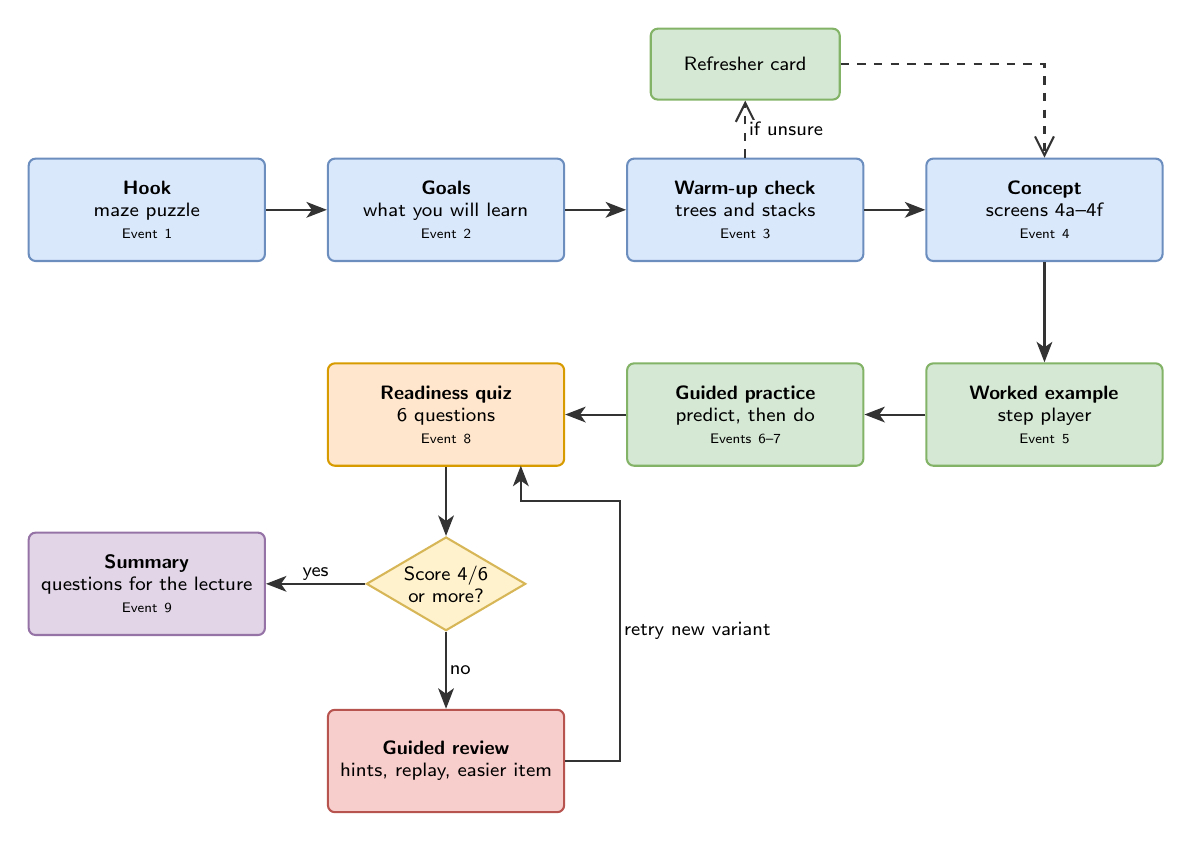
\begin{tikzpicture}[dio, node distance=7mm]
  \tikzset{jb/.style={boxc={#1}{minimum width=30mm, minimum height=13mm, text width=27mm,
                        font=\sffamily\scriptsize}}}
  \node[jb=dioBlue]  (a) at (0,0)     {\textbf{Hook}\\ maze puzzle\\ {\tiny Event 1}};
  \node[jb=dioBlue]  (b) at (3.8,0)   {\textbf{Goals}\\ what you will learn\\ {\tiny Event 2}};
  \node[jb=dioBlue]  (c) at (7.6,0)   {\textbf{Warm-up check}\\ trees and stacks\\ {\tiny Event 3}};
  \node[jb=dioBlue]  (d) at (11.4,0)  {\textbf{Concept}\\ screens 4a--4f\\ {\tiny Event 4}};
  \node[jb=dioGreen] (e) at (11.4,-2.6) {\textbf{Worked example}\\ step player\\ {\tiny Event 5}};
  \node[jb=dioGreen] (f) at (7.6,-2.6)  {\textbf{Guided practice}\\ predict, then do\\ {\tiny Events 6--7}};
  \node[jb=dioOrange] (g) at (3.8,-2.6) {\textbf{Readiness quiz}\\ 6 questions\\ {\tiny Event 8}};
  \node[diamond, aspect=1.7, draw=dioYellowLine, fill=dioYellowFill, font=\sffamily\scriptsize,
        align=center, inner sep=0.3mm] (h) at (3.8,-4.75) {Score 4/6\\ or more?};
  \node[jb=dioPurple] (i) at (0,-4.75)  {\textbf{Summary}\\ questions for the lecture\\ {\tiny Event 9}};
  \node[jb=dioRed]    (j) at (3.8,-7.0) {\textbf{Guided review}\\ hints, replay, easier item};
  \node[boxc={dioGreen}{minimum width=24mm, minimum height=9mm, font=\sffamily\scriptsize}]
        (r) at (7.6,1.85) {Refresher card};
  \draw[arrow] (a) -- (b);
  \draw[arrow] (b) -- (c);
  \draw[arrow] (c) -- (d);
  \draw[arrow] (d) -- (e);
  \draw[arrow] (e) -- (f);
  \draw[arrow] (f) -- (g);
  \draw[arrow] (g) -- (h);
  \draw[arrow] (h) -- node[lbl, above] {yes} (i);
  \draw[arrow] (h) -- node[lbl, right] {no} (j);
  \draw[arrow] (j.east) -- ++(0.7,0) |- node[lbl, pos=0.25, right] {retry new variant} (4.75,-3.7) -- (4.75,-3.25);
  \draw[dep] (c.north) -- node[lbl, right] {if unsure} (r.south);
  \draw[dep] (r.east) -| (d.north);
\end{tikzpicture}}
\caption{Student learning journey. Blue: instruction; green: guided practice; orange: assessment; red: remediation; purple: consolidation.}
\label{fig:journey}
\end{figure}

\subsection{Sequencing principles}

\begin{itemize}
  \item \textbf{Bottom-up through the hierarchy.} Vocabulary and the stack come before DFS; DFS
        search comes before the three traversal orders.
  \item \textbf{Concrete before abstract.} The maze and the plates come before the tree; the tree
        comes before the code; the code is optional.
  \item \textbf{Iterative before recursive.} The explicit stack makes backtracking visible. The
        recursive version is offered afterwards as ``the same thing, with Java keeping the stack
        for you''.
  \item \textbf{Same tree, then new tree.} The worked example uses tree A; practice uses tree B,
        which has a different shape (a node with only one child), so students cannot simply
        memorise a sequence.
  \item \textbf{End with an open question.} The last screen points forward to the lecture rather
        than closing the topic.
\end{itemize}

\subsection{Check against Merrill's First Principles}
\label{sec:merrill}

\begin{tabularx}{\textwidth}{@{}l L@{}}
  \toprule
  \textbf{Principle} & \textbf{Where it appears} \\
  \midrule
  Problem-centred & The session is framed around a real task: finding a value in a tree. \\
  Activation      & Maze hook and warm-up check (Events 1 and 3). \\
  Demonstration   & Worked example in the step player (Event 5). \\
  Application     & Predict mode, the in-order task and the quiz (Events 6 and 8). \\
  Integration     & ``Build your own tree'' sandbox and questions for the lecture (Event 9). \\
  \bottomrule
\end{tabularx}

% =====================================================================
\section{Learning theories and how we apply them}
\label{sec:theory}
% =====================================================================

We did not pick a single theory and force everything through it. Different parts of the session
call for different kinds of learning, so we use each theory where it fits best.

\subsection{Behaviourism: practice with immediate feedback}

Recalling the BST rule and the stack's last-in-first-out behaviour are small, well-defined
responses. For these we use classic behaviourist tools: short questions, immediate confirmation
or correction, and a chance to try again. The warm-up check and the first quiz slot work this way.

\subsection{Cognitivism: managing cognitive load}

DFS asks a beginner to keep track of the tree, the current node, the stack and the output order all
at once, which can easily overload working memory. Cognitive load theory \cite{sweller1988} and
Mayer's multimedia principles \cite{mayer2009} shape the presentation:

\begin{longtable}{@{}p{3.4cm} p{11.4cm}@{}}
  \toprule
  \textbf{Principle} & \textbf{Application in the app} \\
  \midrule
  \endhead
  Segmenting & One step per click; the student controls the pace; nothing plays automatically. \\
  Pre-training & Vocabulary (root, leaf, stack, push, pop) is taught before the algorithm. \\
  Signalling & Colour plus shape shows each node's state: current, visited, on the stack, found. \\
  Spatial contiguity & The explanation sits directly under the tree, and the stack panel directly
                       beside it, so the eye does not have to search. \\
  Coherence & No decorative images, sounds or animations that do not carry meaning. \\
  Redundancy & Narration is text by default. Read-aloud is optional and does not play at the
               same time as on-screen text unless the student switches it on. \\
  Personalisation & Conversational, second-person language (``you'') rather than formal prose. \\
  Worked-example effect & A full worked example before any problem solving, followed by faded
                          practice \cite{atkinson2000}. \\
  \bottomrule
\end{longtable}

\subsection{Constructivism: predict, observe, explain}

Students build understanding by testing their own ideas, not just by receiving ours. In predict
mode the student commits to an answer \emph{before} the app reveals the next step. When the
prediction is wrong, the gap between what they expected and what happened is the moment learning
happens. This follows the predict--observe--explain pattern \cite{white1992}. The ``build your own
tree'' sandbox extends this: students insert their own values and check whether DFS behaves as they
expect.

Research on algorithm visualisation supports this choice. A meta-study by Hundhausen, Douglas and
Stasko \cite{hundhausen2002} found that \emph{how} students engage with a visualisation matters more
than how polished it is, and the engagement taxonomy of Naps et al.\ \cite{naps2002} distinguishes
\emph{viewing} from \emph{responding}, \emph{changing} and \emph{constructing}. The worked example is at
the viewing level, predict mode and the quiz are at the responding level, and the sandbox is at
the changing level.

\subsection{Social constructivism: scaffolding in the zone of proximal development}

Vygotsky's zone of proximal development \cite{vygotsky1978} describes what a learner can do with
help but not yet alone. Scaffolding \cite{wood1976} is the help that bridges that gap and is then
taken away. A real tutor would watch the student, give a small nudge when they are stuck, give
more help if that is not enough, and step back as soon as they cope. The app imitates this with
the hint ladder in Section~\ref{sec:hints} and with the guided review after the quiz. Support is
always offered, never forced, and it fades as the student succeeds.

% =====================================================================
\section{Presentation design}
\label{sec:presentation}
% =====================================================================

\subsection{Visual language}

The same visual language is used on every screen, so that students only have to learn it once.

\begin{figure}[H]
\centering
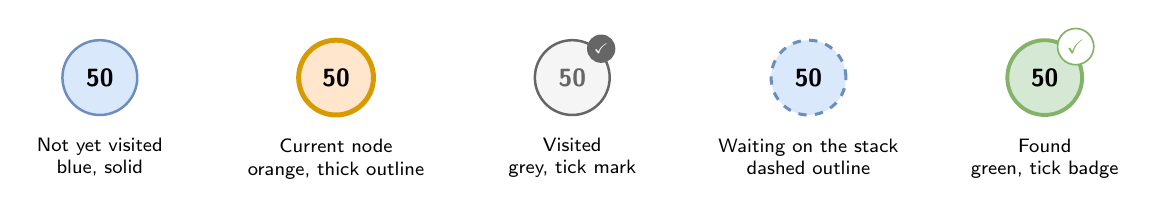
\begin{tikzpicture}[dio]
  \node[treenode]  (u) at (0,0)   {50};
  \node[tcurrent]  (c) at (3,0)   {50};
  \node[tvisited]  (v) at (6,0)   {50};
  \node[tick] at ($(v.north east)+(0.02,0.02)$) {\checkmark};
  \node[tstack]    (s) at (9,0)   {50};
  \node[tfound]    (f) at (12,0)  {50};
  \node[badge, draw=dioGreenLine, fill=white, text=dioGreenLine] at ($(f.north east)+(0.04,0.04)$) {\checkmark};
  \foreach \n/\t in {u/{Not yet visited\\ blue, solid}, c/{Current node\\ orange, thick outline},
                     v/{Visited\\ grey, tick mark}, s/{Waiting on the stack\\ dashed outline},
                     f/{Found\\ green, tick badge}}
    \node[font=\sffamily\scriptsize, align=center, anchor=north] at ($(\n.south)+(0,-0.15)$) {\t};
\end{tikzpicture}
\caption{Node states. Each state differs in shape or outline as well as colour, so colour-blind students can tell them apart.}
\label{fig:legend}
\end{figure}

Colours come from a palette that remains distinguishable under the common forms of colour
blindness. Text meets WCAG AA contrast, and every interactive control can be reached with the Tab
key and used with Enter or Space. Ordering tasks that use drag-and-drop also accept typed input
(for example ``20, 30, 40'') so that keyboard users are not disadvantaged.

\subsection{Writing style}

All learner-facing text follows the same rules:

\begin{itemize}
  \item One idea per screen; no more than about 60 words of explanation at a time.
  \item Short sentences in plain English; technical terms in bold the first time, with a glossary
        tooltip (Appendix~\ref{app:glossary}).
  \item Second person and active voice: ``You visit 30'' rather than ``Node 30 is visited''.
  \item Explanations say \emph{why}, not just \emph{what}: ``30 is on top of the stack, so it comes
        off next.''
  \item Feedback never blames: ``Not quite'' rather than ``Wrong''; mistakes are treated as normal.
\end{itemize}

\subsection{Storyboards}

Figures~\ref{fig:wf-player} and~\ref{fig:wf-quiz} are low-fidelity wireframes of the two most
important screens. They are design targets, not final artwork.

\begin{figure}[H]
\centering
\resizebox{\linewidth}{!}{%
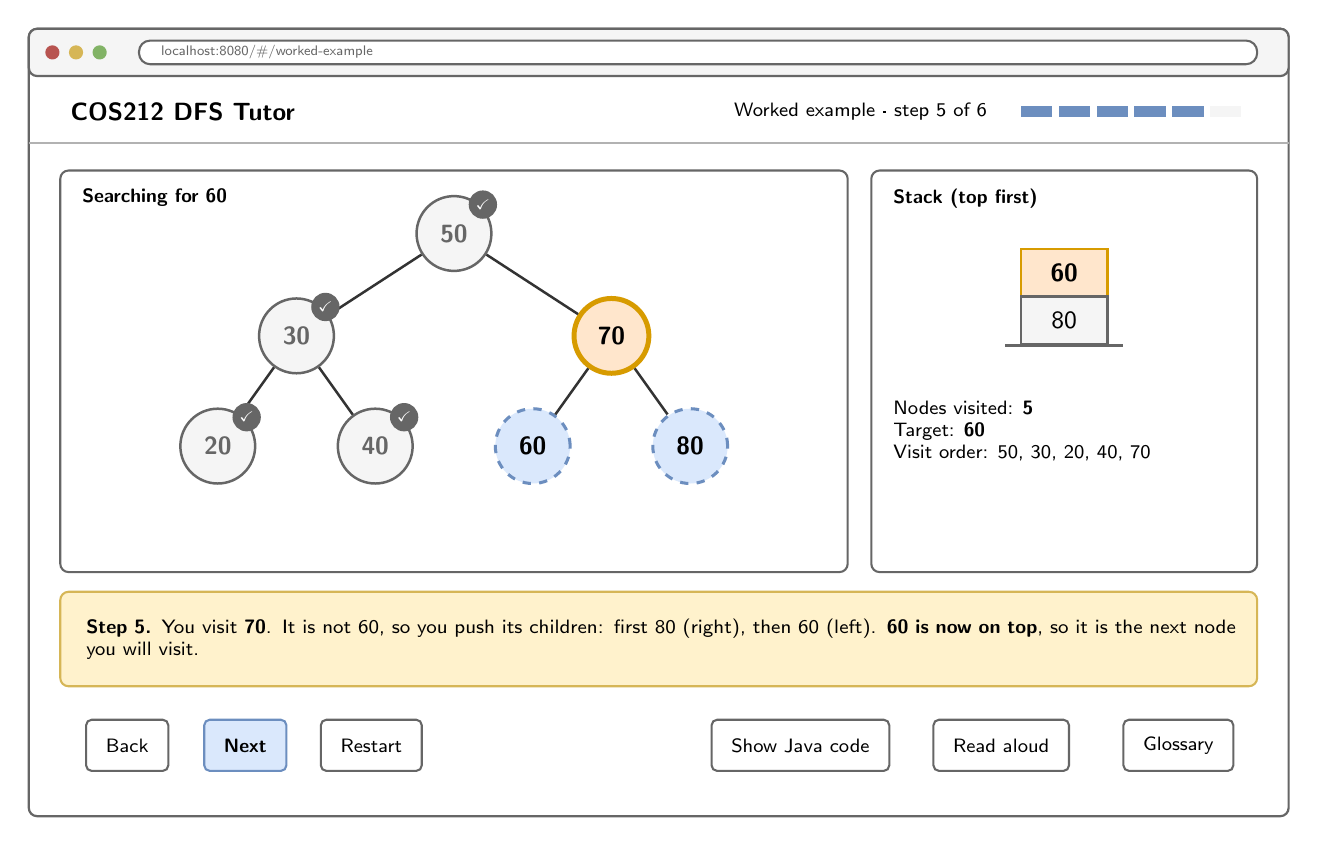
\begin{tikzpicture}[dio]
  \browser{16}{10}{localhost:8080/\#/worked-example}
  % header
  \node[font=\sffamily\small\bfseries, anchor=west] at (0.4,-1.05) {COS212 DFS Tutor};
  \node[font=\sffamily\scriptsize, anchor=east] at (12.3,-1.05) {Worked example \textperiodcentered{} step 5 of 6};
  \foreach \k in {0,...,5} {
    \ifnum\k<5 \def\fc{dioBlueLine}\else\def\fc{dioGreyFill}\fi
    \fill[\fc] ({12.6+\k*0.48},-0.98) rectangle ({12.6+\k*0.48+0.4},-1.12);
  }
  \draw[draw=dioGreyLine!50] (0,-1.45) -- (16,-1.45);
  % tree panel
  \draw[draw=dioGreyLine, rounded corners=3pt] (0.4,-1.8) rectangle (10.4,-6.9);
  \node[font=\sffamily\scriptsize\bfseries, anchor=north west] at (0.55,-1.9) {Searching for 60};
  \node[tvisited] (a50) at (5.4,-2.6) {50};
  \node[tvisited] (a30) at (3.4,-3.9) {30};
  \node[tcurrent] (a70) at (7.4,-3.9) {70};
  \node[tvisited] (a20) at (2.4,-5.3) {20};
  \node[tvisited] (a40) at (4.4,-5.3) {40};
  \node[tstack]   (a60) at (6.4,-5.3) {60};
  \node[tstack]   (a80) at (8.4,-5.3) {80};
  \foreach \p/\c in {a50/a30, a50/a70, a30/a20, a30/a40, a70/a60, a70/a80}
    \draw[draw=edge, line width=0.9pt] (\p) -- (\c);
  \foreach \n in {a50,a30,a20,a40} \node[tick] at ($(\n.north east)+(0.02,0.02)$) {\checkmark};
  % stack panel
  \draw[draw=dioGreyLine, rounded corners=3pt] (10.7,-1.8) rectangle (15.6,-6.9);
  \node[font=\sffamily\scriptsize\bfseries, anchor=north west] at (10.85,-1.9) {Stack (top first)};
  \node[stktop] at (13.15,-3.1) {60};
  \node[stk]    at (13.15,-3.7) {80};
  \draw[draw=dioGreyLine, line width=0.9pt] (12.4,-4.02) -- (13.9,-4.02);
  \node[font=\sffamily\scriptsize, align=left, anchor=north west] at (10.85,-4.6)
       {Nodes visited: \textbf{5}\\ Target: \textbf{60}\\ Visit order: 50, 30, 20, 40, 70};
  % explanation
  \draw[draw=dioYellowLine, fill=dioYellowFill, rounded corners=3pt] (0.4,-7.15) rectangle (15.6,-8.35);
  \node[font=\sffamily\scriptsize, align=left, anchor=west, text width=14.6cm] at (0.6,-7.75)
       {\textbf{Step 5.} You visit \textbf{70}. It is not 60, so you push its children: first 80
        (right), then 60 (left). \textbf{60 is now on top}, so it is the next node you will visit.};
  % controls
  \node[wfbtn]  at (1.25,-9.1)  {Back};
  \node[wfbtnp] at (2.75,-9.1)  {Next};
  \node[wfbtn]  at (4.35,-9.1)  {Restart};
  \node[wfbtn]  at (9.8,-9.1)   {Show Java code};
  \node[wfbtn]  at (12.35,-9.1) {Read aloud};
  \node[wfbtn]  at (14.6,-9.1)  {Glossary};
\end{tikzpicture}}
\caption{Wireframe of the step player during the worked example (step 5 of the search for 60).}
\label{fig:wf-player}
\end{figure}

\begin{figure}[H]
\centering
\resizebox{\linewidth}{!}{%
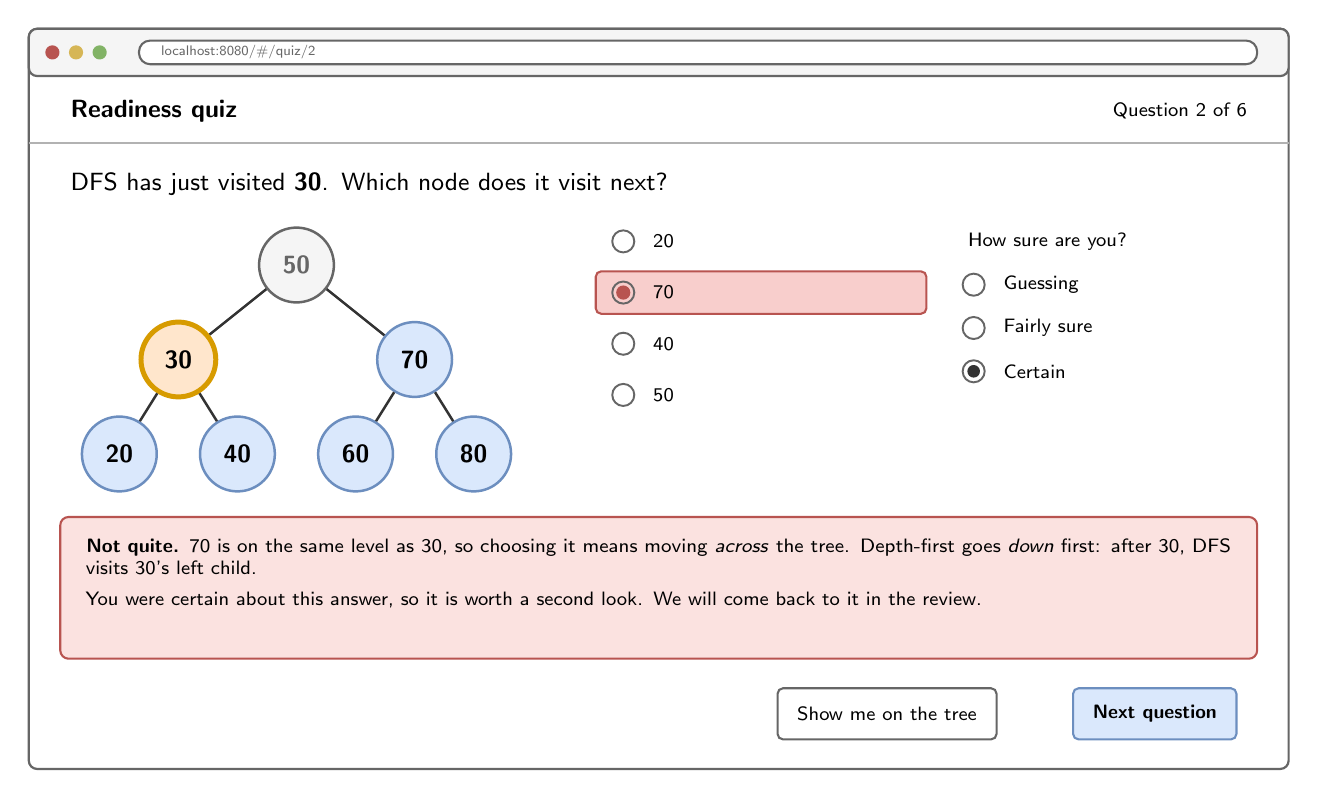
\begin{tikzpicture}[dio]
  \browser{16}{9.4}{localhost:8080/\#/quiz/2}
  \node[font=\sffamily\small\bfseries, anchor=west] at (0.4,-1.05) {Readiness quiz};
  \node[font=\sffamily\scriptsize, anchor=east] at (15.6,-1.05) {Question 2 of 6};
  \draw[draw=dioGreyLine!50] (0,-1.45) -- (16,-1.45);
  \node[font=\sffamily\small, anchor=north west, text width=15cm] at (0.4,-1.7)
       {DFS has just visited \textbf{30}. Which node does it visit next?};
  % tree
  \node[tvisited] (q50) at (3.4,-3.0) {50};
  \node[tcurrent] (q30) at (1.9,-4.2) {30};
  \node[treenode] (q70) at (4.9,-4.2) {70};
  \node[treenode] (q20) at (1.15,-5.4) {20};
  \node[treenode] (q40) at (2.65,-5.4) {40};
  \node[treenode] (q60) at (4.15,-5.4) {60};
  \node[treenode] (q80) at (5.65,-5.4) {80};
  \foreach \p/\c in {q50/q30, q50/q70, q30/q20, q30/q40, q70/q60, q70/q80}
    \draw[draw=edge, line width=0.9pt] (\p) -- (\c);
  % options
  \foreach \y/\t/\sel in {-2.7/20/0, -3.35/70/1, -4.0/40/0, -4.65/50/0} {
    \ifnum\sel=1
      \draw[draw=dioRedLine, fill=dioRedFill, rounded corners=2pt] (7.2,{\y+0.27}) rectangle (11.4,{\y-0.27});
      \fill[dioRedLine] (7.55,\y) circle (0.09);
    \fi
    \draw[draw=dioGreyLine, line width=0.7pt] (7.55,\y) circle (0.14);
    \node[font=\sffamily\scriptsize, anchor=west] at (7.8,\y) {\t};
  }
  \node[font=\sffamily\scriptsize, anchor=west] at (11.8,-2.7) {How sure are you?};
  \foreach \y/\t/\sel in {-3.25/Guessing/0, -3.8/Fairly sure/0, -4.35/Certain/1} {
    \draw[draw=dioGreyLine, line width=0.7pt] (12.0,\y) circle (0.14);
    \ifnum\sel=1 \fill[edge] (12.0,\y) circle (0.08); \fi
    \node[font=\sffamily\scriptsize, anchor=west] at (12.25,\y) {\t};
  }
  % feedback
  \draw[draw=dioRedLine, fill=dioRedFill!60, rounded corners=3pt] (0.4,-6.2) rectangle (15.6,-8.0);
  \node[font=\sffamily\scriptsize, align=left, anchor=north west, text width=14.6cm] at (0.6,-6.35)
       {\textbf{Not quite.} 70 is on the same level as 30, so choosing it means moving
        \emph{across} the tree. Depth-first goes \emph{down} first: after 30, DFS visits 30's
        left child.\\[3pt]
        You were certain about this answer, so it is worth a second look. We will come back to it
        in the review.};
  \node[wfbtn]  at (10.9,-8.7) {Show me on the tree};
  \node[wfbtnp] at (14.3,-8.7) {Next question};
\end{tikzpicture}}
\caption{Wireframe of a quiz question after a confident wrong answer (misconception M1).}
\label{fig:wf-quiz}
\end{figure}

% =====================================================================
\section{Catering for different learners}
\label{sec:styles}
% =====================================================================

\subsection{Learning styles: what we do and what we do not claim}

The specification asks which learning styles the app caters for. The best known model is VARK
(Visual, Aural, Read/write, Kinaesthetic) \cite{fleming1992}, and we map our features onto it below.
However, we want to be careful. A widely cited review by Pashler et al.\ \cite{pashler2008} found
little evidence that teaching to a student's \emph{preferred} style improves learning. Our design
therefore does not try to diagnose a student's style and adapt to it. Instead, every student gets
several representations of the same idea, which research on multimedia learning does support
\cite{mayer2009}. Students who prefer one mode will still find it, and all students benefit from
seeing the idea more than one way.

\begin{longtable}{@{}p{2.6cm} p{12.2cm}@{}}
  \toprule
  \textbf{VARK mode} & \textbf{How the app provides it} \\
  \midrule
  \endhead
  Visual & Tree diagram with colour and shape states; animated stack panel; maze picture on the
           hook screen; side-by-side comparison of the three orders. \\
  Aural & Optional read-aloud of each explanation using the browser's built-in speech
          synthesis. \\
  Read/write & Short written explanations on every step; glossary tooltips; summary screen that
               can be printed; optional Java code view. \\
  Kinaesthetic & Clicking through steps at their own pace; predicting the next node; dragging
                 nodes into order; inserting values and watching the tree grow. \\
  \bottomrule
\end{longtable}

\subsection{Universal Design for Learning}

We also check the design against the three principles of Universal Design for Learning
\cite{cast2018}, which are about designing for the whole range of learners from the start:

\begin{itemize}
  \item \textbf{Multiple means of engagement:} the student chooses the pace, can skip refresher
        material they do not need, and can explore their own trees in the sandbox.
  \item \textbf{Multiple means of representation:} picture, stack, text, optional audio and
        optional code, as above.
  \item \textbf{Multiple means of action and expression:} answers can be given by clicking a node,
        choosing an option, dragging or typing.
\end{itemize}

\subsection{Different starting points}

Some students will already know a little about trees; others will not know what a stack is. The
warm-up check handles this. A student who answers both warm-up questions correctly goes straight on;
a student who misses one sees the matching refresher card (about one minute each). This keeps the
session short for students who are ready while still honouring the requirement that no prior
knowledge is assumed.

% =====================================================================
\section{Motivation}
\label{sec:motivation}
% =====================================================================

Because the app carries no marks, students need reasons of their own to start it and finish it.
We use Keller's ARCS model \cite{keller1987} to design for this deliberately.

\begin{longtable}{@{}p{2.3cm} p{6.4cm} p{6.1cm}@{}}
  \toprule
  \textbf{ARCS} & \textbf{Tactic} & \textbf{Where in the app} \\
  \midrule
  \endhead
  \textbf{Attention} & Open with a puzzle rather than a definition. & Hook screen (maze). \\
   & Create small moments of suspense: ``What do you think comes next?'' & Predict mode. \\
   & Vary the activity every few minutes (read, watch, predict, drag, answer). & Whole journey. \\
  \textbf{Relevance} & Connect to familiar things: folders inside folders, exploring a maze, the
       undo button (a stack). & Concept screens 4b and 4c. \\
   & Say plainly how this helps: ``The lecture will build on this. Doing it now makes the lecture
     easier to follow.'' & Goals screen. \\
  \textbf{Confidence} & Clear goals and a visible progress bar. & Every screen. \\
   & Early, easy wins before harder tasks. & Warm-up, then worked example, then practice. \\
   & Hints instead of dead ends; mistakes framed as normal. & Hint ladder, feedback wording. \\
   & Honest, low-stakes readiness check. & Quiz with no marks recorded. \\
  \textbf{Satisfaction} & Immediate feedback that recognises correct reasoning, not just the right
       answer. & Feedback panel. \\
   & A genuine ``aha'' moment: the in-order output is sorted. & Screen 4e. \\
   & A summary of what they can now do, and questions to take to the lecture. & Summary screen. \\
  \bottomrule
\end{longtable}

We considered points, badges and leaderboards and decided against them for this prototype.
Extrinsic rewards can crowd out interest in the material itself, a leaderboard would require
accounts and stored data, and both would take development time away from feedback quality, which
matters more for learning.

% =====================================================================
\section{Assessment, feedback and scaffolding}
\label{sec:assess}
% =====================================================================

\subsection{Purpose of assessment in a pre-lecture app}

All assessment in the app is \textbf{formative}: its job is to help the student learn and to give
them an honest picture of their readiness, not to grade them. There are three kinds:

\begin{tabularx}{\textwidth}{@{}l l L@{}}
  \toprule
  \textbf{Type} & \textbf{When} & \textbf{Purpose} \\
  \midrule
  Diagnostic  & Warm-up check (Event 3) & Find missing prerequisites and route to a refresher. \\
  Embedded    & Predict mode and practice (Event 6) & Practise with immediate feedback and hints. \\
  Summative-style & Readiness quiz (Event 8) & Decide whether to offer guided review. Nothing is recorded. \\
  \bottomrule
\end{tabularx}

\subsection{The readiness quiz}

The quiz has six \emph{slots}, each tied to a learning outcome. Every slot has at least two
equivalent items (variant A and variant B) in the bank, and a third variant can be generated by
relabelling the values of the tree while keeping its shape, with the correct answers calculated by
the Java backend. A first attempt draws variant A; a retry draws a variant the student has not
seen. The full bank, with every option and its feedback, is in Appendix~\ref{app:quiz}.

\begin{tabularx}{\textwidth}{@{}c c l L@{}}
  \toprule
  \textbf{Slot} & \textbf{LO} & \textbf{Bloom} & \textbf{Item format} \\
  \midrule
  1 & LO1 & Remember   & Multiple choice \\
  2 & LO2 & Understand & Click the node on the tree, or multiple choice \\
  3 & LO3 & Apply      & Put the nodes in order (drag or type) \\
  4 & LO4 & Apply      & Multiple choice about stack contents \\
  5 & LO5 & Analyse    & Multiple choice: how many nodes are visited \\
  6 & LO5 & Analyse    & Multiple choice: explain why \\
  \bottomrule
\end{tabularx}

Wrong options are not random. Each one is built from a specific misconception (M1--M5), so the
feedback can explain the actual error in the student's thinking.

\textbf{Confidence rating.} After each answer the student says how sure they were: guessing,
fairly sure or certain. This does not change the score. It helps students reflect on what they
really know, and it helps the app prioritise: a \emph{confident wrong} answer suggests a firmly held
misconception and is reviewed first; a \emph{guessed right} answer is flagged as ``worth another
look'' in the summary.

\subsection{Feedback design}

Feedback is written to answer the three questions Hattie and Timperley identify as making feedback
effective \cite{hattie2007}: \emph{Where am I going? How am I going? Where to next?} Shute's review of
formative feedback \cite{shute2008} adds practical guidance that we follow: be specific, focus on the
task rather than the person, keep it short, and give it immediately for novices.

Every feedback message therefore has the same three parts:

\begin{enumerate}
  \item \textbf{Verdict:} ``Correct'' or ``Not quite''.
  \item \textbf{Reason:} why the answer is right, or which idea led to the wrong answer.
  \item \textbf{Next move:} what to look at, or what to try next time.
\end{enumerate}

Correct answers get feedback too. A student may be right for the wrong reason, so the reason is
always stated.

\subsection{Hint ladder in guided practice}
\label{sec:hints}

When a student makes a wrong prediction in practice, the app does not simply give the answer. It
climbs a three-step ladder, giving only as much help as is needed (Figure~\ref{fig:hints}).

\begin{tabularx}{\textwidth}{@{}l l L@{}}
  \toprule
  \textbf{Level} & \textbf{Type} & \textbf{Example (predicting the node after 50)} \\
  \midrule
  1 & Attention nudge & ``Look at the stack. Which node is on top?'' \\
  2 & Rule reminder   & ``DFS always takes the top node off the stack. After 50 we pushed 70, then 30.
                         Which went on last?'' \\
  3 & Worked answer   & ``The next node is 30. It was pushed last, so it is on top and comes off
                         first. That is why DFS explores the left side before the right.'' \\
  \bottomrule
\end{tabularx}

\begin{figure}[H]
\centering
\resizebox{\linewidth}{!}{%
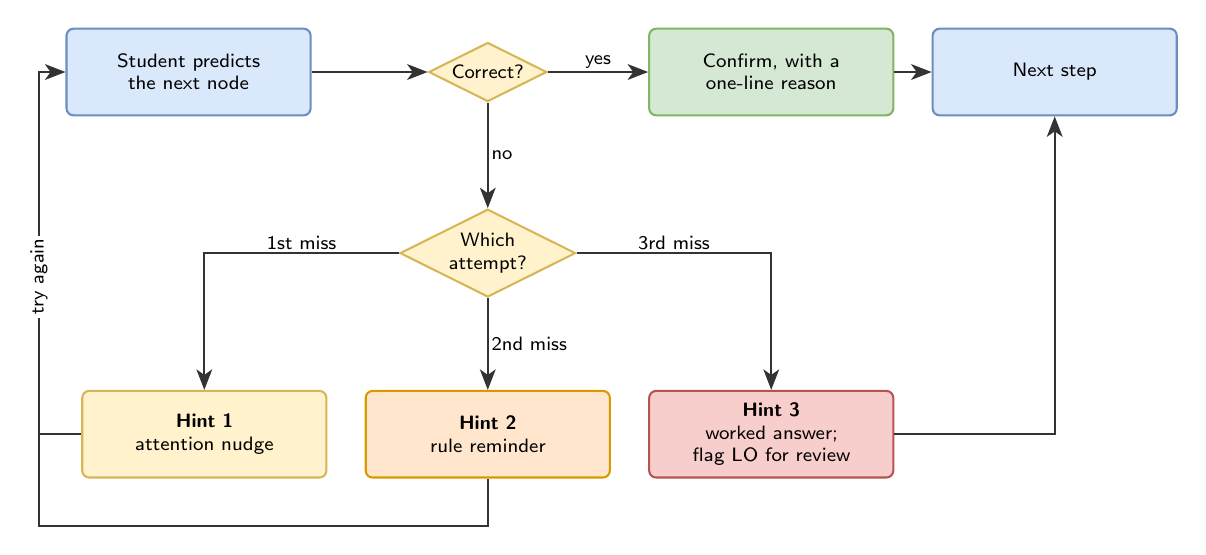
\begin{tikzpicture}[dio, font=\sffamily\scriptsize]
  \tikzset{hb/.style={boxc={#1}{minimum width=30mm, text width=28mm, minimum height=11mm, font=\sffamily\scriptsize}},
           dec/.style={diamond, aspect=2.0, draw=dioYellowLine, fill=dioYellowFill, align=center,
                       inner sep=0.4mm, font=\sffamily\scriptsize}}
  \node[hb=dioBlue]   (p)  at (0,0)     {Student predicts the next node};
  \node[dec]          (d1) at (3.8,0)   {Correct?};
  \node[hb=dioGreen]  (ok) at (7.4,0)   {Confirm, with a one-line reason};
  \node[hb=dioBlue]   (nx) at (11.0,0)  {Next step};
  \node[dec]          (d2) at (3.8,-2.3) {Which\\ attempt?};
  \node[hb=dioYellow] (h1) at (0.2,-4.6)  {\textbf{Hint 1}\\ attention nudge};
  \node[hb=dioOrange] (h2) at (3.8,-4.6)  {\textbf{Hint 2}\\ rule reminder};
  \node[hb=dioRed]    (h3) at (7.4,-4.6)  {\textbf{Hint 3}\\ worked answer; flag LO for review};
  \draw[arrow] (p) -- (d1);
  \draw[arrow] (d1) -- node[lbl, above] {yes} (ok);
  \draw[arrow] (ok) -- (nx);
  \draw[arrow] (d1) -- node[lbl, right] {no} (d2);
  \draw[arrow] (d2.west) -| node[lbl, pos=0.25, above] {1st miss} (h1.north);
  \draw[arrow] (d2) -- node[lbl, right] {2nd miss} (h2);
  \draw[arrow] (d2.east) -| node[lbl, pos=0.25, above] {3rd miss} (h3.north);
  \draw[draw=edge, line width=0.75pt] (h1.west) -- (-1.9,-4.6);
  \draw[arrow] (h2.south) -- ++(0,-0.6) -| (-1.9,-1.0) |- (p.west);
  \draw[arrow] (h3.east) -| (nx.south);
  \node[lbl, rotate=90] at (-1.9,-2.6) {try again};
\end{tikzpicture}}
\caption{How the app responds to a prediction in guided practice.}
\label{fig:hints}
\end{figure}

If a student reaches hint 3 twice in the same practice, the app suggests replaying the worked
example before continuing. It does not insist.

\subsection{Scaffolding after the quiz}

The quiz outcome decides what is \emph{offered} next:

\begin{itemize}
  \item \textbf{4/6 or more:} the student goes to the summary screen. Any item they got wrong, or
        guessed right, is listed with a link to the relevant screen.
  \item \textbf{Below 4/6:} the app offers a guided review built from the outcomes they missed,
        confident wrong answers first. For each missed outcome it (1) replays the relevant part of
        the worked example with the reason highlighted, (2) asks an easier version of the question
        with hint 1 already shown, and (3) explains the answer. The student then takes a fresh
        variant of the quiz.
\end{itemize}

The student can always choose ``Continue to summary anyway''. They are adults managing their own
preparation, and a forced loop would hurt motivation more than it helps.

\textbf{Why 4/6?} Two correct answers in six could be luck, and slots 5 and 6 are the hardest. A
score of 4 or more means the student has at least shown the core Apply-level skills. This is a
starting value; Section~\ref{sec:eval} explains how we will check it.

% =====================================================================
\section{Development}
\label{sec:dev}
% =====================================================================

\subsection{Content production}

\begin{enumerate}
  \item Lesson text and quiz items are written in JSON files (\code{lesson.json},
        \code{quiz-bank.json}) so that ID work and code can proceed in parallel.
  \item Every quiz answer and every number quoted in a lesson (visit orders, stack contents,
        node counts) is checked against the output of the Java implementation. The backend's unit
        tests include the trees used in the lesson.
  \item Two group members who did not write an item review it against a checklist: aligned to its
        outcome, one clearly correct answer, each distractor tied to a misconception, feedback
        follows verdict--reason--next move, no more than about 60 words.
  \item Wording is read aloud once to catch long or awkward sentences.
\end{enumerate}

\subsection{Example trees}

\begin{tabularx}{\textwidth}{@{}l L L@{}}
  \toprule
  & \textbf{Tree A (worked example)} & \textbf{Tree B (practice)} \\
  \midrule
  Inserted in order & 50, 30, 70, 20, 40, 60, 80 & 45, 25, 65, 15, 35, 55, 30 \\
  Shape & Perfect: every internal node has two children & Uneven: 35 has only a left child, 65 only a left child \\
  Pre-order  & 50, 30, 20, 40, 70, 60, 80 & 45, 25, 15, 35, 30, 65, 55 \\
  In-order   & 20, 30, 40, 50, 60, 70, 80 & 15, 25, 30, 35, 45, 55, 65 \\
  Post-order & 20, 40, 30, 60, 80, 70, 50 & 15, 30, 35, 25, 55, 65, 45 \\
  Search used & 60: found after 6 visits & 55: found after 7 visits \\
  \bottomrule
\end{tabularx}

\begin{figure}[H]
\centering
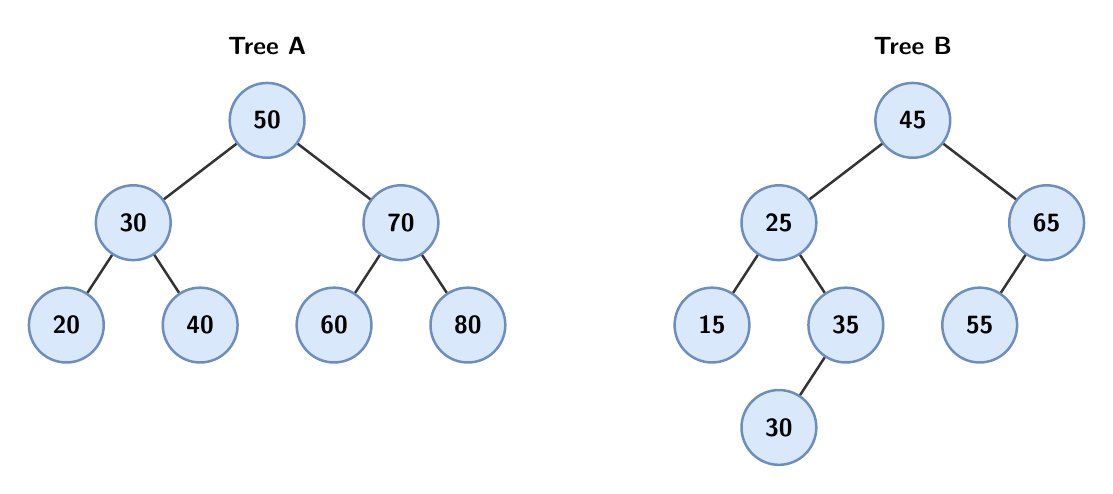
\begin{tikzpicture}[dio, level distance=13mm,
    every child node/.style={treenode},
    edge from parent/.style={draw=edge, line width=0.9pt}]
  \begin{scope}[level 1/.style={sibling distance=34mm}, level 2/.style={sibling distance=17mm}]
  \node[treenode] {50}
    child {node {30} child {node {20}} child {node {40}}}
    child {node {70} child {node {60}} child {node {80}}};
  \node[font=\sffamily\small\bfseries] at (0,0.95) {Tree A};
  \end{scope}
  \begin{scope}[xshift=8.2cm, level 1/.style={sibling distance=34mm}, level 2/.style={sibling distance=17mm}]
  \node[treenode] {45}
    child {node {25}
      child {node {15}}
      child {node {35} child {node {30}} child[missing]}}
    child {node {65}
      child {node {55}}
      child[missing]};
  \node[font=\sffamily\small\bfseries] at (0,0.95) {Tree B};
  \end{scope}
\end{tikzpicture}
\caption{The two trees used in the lesson. Tree B's uneven shape stops students memorising a fixed pattern.}
\label{fig:trees}
\end{figure}

\subsection{Trace of the practice search}

Practice 1 asks students to predict each step of a DFS search for 55 on tree B. The expected
answers, which the feedback is built on, are:

\begin{tabularx}{\textwidth}{@{}c c L l@{}}
  \toprule
  \textbf{Step} & \textbf{Visit} & \textbf{What happens} & \textbf{Stack after (top first)} \\
  \midrule
  1 & 45 & Not 55. Push 65, then 25. & 25, 65 \\
  2 & 25 & Not 55. Push 35, then 15. & 15, 35, 65 \\
  3 & 15 & Leaf. Backtrack. & 35, 65 \\
  4 & 35 & Not 55. Only a left child: push 30. & 30, 65 \\
  5 & 30 & Leaf. Backtrack. & 65 \\
  6 & 65 & Not 55. Only a left child: push 55. & 55 \\
  7 & 55 & Found. Stop. & (empty) \\
  \bottomrule
\end{tabularx}

Step 4 is deliberately interesting: a node with only one child tests whether students really
understand ``skip empty children'' or are just alternating left and right.

% =====================================================================
\section{Implementation}
\label{sec:impl}
% =====================================================================

\subsection{Delivery to students}

In a real rollout the lecturer would post the link on ClickUP two or three days before the lecture
on tree traversal, with a one-line message: ``Spend 20 minutes on this before Thursday's lecture.
It is not marked.'' For the prototype the app runs locally (see the SE document), so delivery is
limited to the peer pilot and the examination demonstration.

\subsection{Guidance for the lecturer}

\begin{itemize}
  \item The app assumes no prior knowledge, so it can be set before the topic is introduced.
  \item The summary screen ends with two questions. Opening the lecture with them connects the
        lecture directly to what students did:
        \begin{enumerate}
          \item ``DFS needed six visits to find 60. Using the BST rule it needs only three. How,
                and what is the worst case?''
          \item ``When would you rather explore level by level instead of depth first?''
        \end{enumerate}
  \item The prototype records nothing. A later version could report anonymous, class-level quiz
        results so the lecturer can see which misconceptions are most common.
\end{itemize}

\subsection{Examination demonstration}

The ten-minute demonstration follows one student's path through the app: hook, one concept screen,
the worked example, a wrong prediction showing the hint ladder, a quiz question answered wrongly
with confidence, and the guided review. This shows the instructional design working, not just the
software.

% =====================================================================
\section{Evaluation}
\label{sec:eval}
% =====================================================================

\subsection{Evaluation questions}

\begin{enumerate}
  \item Do students learn DFS from the app? (Kirkpatrick level 2, learning \cite{kirkpatrick2006})
  \item Do students find it usable and worth their time? (level 1, reaction)
  \item Which screens or questions cause confusion?
  \item Is the 4/6 threshold a sensible point at which to offer guided review?
\end{enumerate}

Levels 3 and 4 (behaviour in the lecture and results in the module) cannot be measured within the
examination timeline; Section~\ref{sec:reflect} discusses how they could be measured later.

\subsection{Formative evaluation plan}

Following the staged approach of Dick and Carey's formative evaluation, we evaluate in three rounds:

\begin{longtable}{@{}p{2.6cm} p{2.4cm} p{6.0cm} p{3.6cm}@{}}
  \toprule
  \textbf{Round} & \textbf{When} & \textbf{What we do} & \textbf{Changes allowed} \\
  \midrule
  \endhead
  Expert review & 4--5 Nov & A COS212 tutor checks the lesson text and quiz bank for accuracy and
      level. & Content corrections. \\
  One-to-one & 8 Nov & Two students who have not done COS212 use the app while thinking aloud; a
      group member observes and takes notes. & Wording, layout, hints. \\
  Small group & 9 Nov & Three to five students use the app independently and complete the
      instruments below. & Fixes only; no new features. \\
  \bottomrule
\end{longtable}

\subsection{Instruments}

\begin{itemize}
  \item \textbf{Pre-test and post-test:} five short questions, in two parallel forms, taken before
        and after the session (Appendix~\ref{app:eval}). Using different forms avoids simply
        measuring memory of the first test.
  \item \textbf{System Usability Scale (SUS):} the standard ten-item questionnaire \cite{brooke1996}.
  \item \textbf{Three open questions:} what helped most, what was confusing, what they would change.
  \item \textbf{Observation checklist:} where the student hesitates, uses hints, goes back, or
        says something unexpected.
  \item \textbf{Session time:} start and finish time.
\end{itemize}

\subsection{Success criteria}

The pilot is small, so these figures are indicators, not proof. We will consider the design to be
working if:

\begin{itemize}
  \item the average post-test score is at least two points higher than the pre-test score (out of
        five), and no student scores lower;
  \item the average SUS score is 68 or above (the commonly used benchmark for ``above average'');
  \item the median session time is between 15 and 30 minutes;
  \item no single screen is marked as confusing by more than one participant.
\end{itemize}

\textbf{Checking the threshold.} If students who scored 3/6 on the quiz do as well on the post-test
as those who scored 4/6, the threshold is too high; if students who scored 4/6 still do poorly on
the post-test, it is too low. With a small pilot this can only point in a direction, but it is
better than leaving the number untested.

% =====================================================================
\section{Reflection on our instructional choices}
\label{sec:reflect}
% =====================================================================

The specification asks us to reflect on our choices, not only to describe them. These are the
decisions we debated most, and the trade-offs we accepted.

\paragraph{DFS on a tree rather than on a graph.} On a tree, DFS does not need a ``visited'' set
because there are no cycles. This makes the first encounter much simpler, but it means students do
not yet meet the part of DFS that matters most for graphs. We think this is the right order: one
new idea at a time. The lecture can add the visited set as the next step, and our summary
questions point towards it.

\paragraph{Iterative stack first, recursion second.} Showing the explicit stack makes backtracking
visible, which directly addresses misconception M2. The cost is that the traversal orders are
easiest to explain recursively, so students see two versions. We reduce the risk by showing the
recursive call stack in the same stack panel and by saying explicitly that it is the same idea.
We will watch for confusion here in the pilot.

\paragraph{Learning styles.} We were asked about learning styles, and VARK is familiar to students
and lecturers, so we used it to organise our thinking. But we chose not to build ``style
detection'', because the evidence does not support it \cite{pashler2008}. Giving everyone multiple
representations is cheaper to build, better supported by research, and fairer.

\paragraph{No gamification.} Points and badges would make a stronger first impression in a demo.
We decided that time spent on precise, misconception-based feedback would do more for learning.
This may make the app look plainer than some others; we accept that.

\paragraph{Offering, not forcing, remediation.} A forced remediation loop guarantees that students
see the review, but it treats them as if they cannot judge their own needs and can be frustrating.
We chose to offer it, using the confidence rating to make the recommendation persuasive. Whether
students actually take it up is something the pilot should tell us.

\paragraph{What the prototype cannot do yet.} Without accounts or stored data we cannot offer
spaced practice (coming back to the topic a few days later), which is one of the most reliable
ways to improve long-term retention. We also cannot measure Kirkpatrick levels 3 and 4. Both would
be natural next steps: a short follow-up quiz a week after the lecture, and anonymous class-level
results for the lecturer.

% =====================================================================
\begin{thebibliography}{99}
\bibitem{anderson2001} L.\,W. Anderson and D.\,R. Krathwohl (eds.). \emph{A Taxonomy for Learning,
  Teaching, and Assessing: A Revision of Bloom's Taxonomy of Educational Objectives}. Longman, 2001.
\bibitem{atkinson2000} R.\,K. Atkinson, S.\,J. Derry, A. Renkl and D. Wortham. Learning from examples:
  instructional principles from the worked examples research. \emph{Review of Educational Research},
  70(2):181--214, 2000.
\bibitem{biggs1996} J. Biggs. Enhancing teaching through constructive alignment. \emph{Higher
  Education}, 32(3):347--364, 1996.
\bibitem{branch2009} R.\,M. Branch. \emph{Instructional Design: The ADDIE Approach}. Springer, 2009.
\bibitem{brooke1996} J. Brooke. SUS: a ``quick and dirty'' usability scale. In P.\,W. Jordan et al.
  (eds.), \emph{Usability Evaluation in Industry}, pp.\ 189--194. Taylor \& Francis, 1996.
\bibitem{cast2018} CAST. \emph{Universal Design for Learning Guidelines}, version 2.2. 2018.
  \url{http://udlguidelines.cast.org}
\bibitem{cs2023} A.\,N. Kumar, R.\,K. Raj, S.\,G. Aly, M.\,D. Anderson, B.\,A. Becker et al.
  \emph{Computer Science Curricula 2023}. Association for Computing Machinery, New York, 2024.
\bibitem{fleming1992} N.\,D. Fleming and C. Mills. Not another inventory, rather a catalyst for
  reflection. \emph{To Improve the Academy}, 11:137--155, 1992.
\bibitem{gagne2005} R.\,M. Gagn\'e, W.\,W. Wager, K.\,C. Golas and J.\,M. Keller.
  \emph{Principles of Instructional Design}, 5th ed. Wadsworth, 2005.
\bibitem{hattie2007} J. Hattie and H. Timperley. The power of feedback. \emph{Review of Educational
  Research}, 77(1):81--112, 2007.
\bibitem{hundhausen2002} C.\,D. Hundhausen, S.\,A. Douglas and J.\,T. Stasko. A meta-study of
  algorithm visualization effectiveness. \emph{Journal of Visual Languages and Computing},
  13(3):259--290, 2002.
\bibitem{keller1987} J.\,M. Keller. Development and use of the ARCS model of instructional design.
  \emph{Journal of Instructional Development}, 10(3):2--10, 1987.
\bibitem{kirkpatrick2006} D.\,L. Kirkpatrick and J.\,D. Kirkpatrick. \emph{Evaluating Training
  Programs: The Four Levels}, 3rd ed. Berrett-Koehler, 2006.
\bibitem{mayer2009} R.\,E. Mayer. \emph{Multimedia Learning}, 2nd ed. Cambridge University Press, 2009.
\bibitem{merrill2002} M.\,D. Merrill. First principles of instruction. \emph{Educational Technology
  Research and Development}, 50(3):43--59, 2002.
\bibitem{naps2002} T.\,L. Naps, G. R\"o{\ss}ling et al. Exploring the role of visualization and
  engagement in computer science education. \emph{ACM SIGCSE Bulletin}, 35(2):131--152, 2003
  (ITiCSE 2002 working group report).
\bibitem{pashler2008} H. Pashler, M. McDaniel, D. Rohrer and R. Bjork. Learning styles: concepts
  and evidence. \emph{Psychological Science in the Public Interest}, 9(3):105--119, 2008.
\bibitem{shute2008} V.\,J. Shute. Focus on formative feedback. \emph{Review of Educational Research},
  78(1):153--189, 2008.
\bibitem{sweller1988} J. Sweller. Cognitive load during problem solving: effects on learning.
  \emph{Cognitive Science}, 12(2):257--285, 1988.
\bibitem{vygotsky1978} L.\,S. Vygotsky. \emph{Mind in Society: The Development of Higher
  Psychological Processes}. Harvard University Press, 1978.
\bibitem{white1992} R. White and R. Gunstone. \emph{Probing Understanding}. Falmer Press, 1992.
\bibitem{wood1976} D. Wood, J.\,S. Bruner and G. Ross. The role of tutoring in problem solving.
  \emph{Journal of Child Psychology and Psychiatry}, 17(2):89--100, 1976.
\end{thebibliography}

% =====================================================================
\appendix
% =====================================================================

\section{Lesson script}
\label{app:script}

This is the text the student sees, screen by screen. Words in bold link to the glossary.

\subsection*{Screen 1: Hook (Event 1)}
\begin{quote}\sffamily\small
You are standing at the entrance of a maze. You can only see the passage right in front of you.
At each fork you must choose a way to go.\\[4pt]
\textbf{How would you make sure you never miss the exit?}\\
( ) Pick a random passage every time.\\
( ) Always take the left-most passage you have not tried yet. If you hit a dead end, go back to
the last fork and try the next passage.\\
( ) Try the first step of every passage, then the second step of every passage, and so on.\\[4pt]
\emph{After any choice:} All three are real strategies, and two of them always work. Today you will
learn the second one. It is called \textbf{depth-first search}.
\end{quote}

\subsection*{Screen 2: Goals (Event 2)}
\begin{quote}\sffamily\small
In the next 20 minutes you will learn to:\\
1. Walk through a tree the depth-first way, and explain what that means.\\
2. Use a \textbf{stack} to keep track of where to go back to.\\
3. Check whether you are ready for the lecture, and get help if you are not.\\[4pt]
You can go back to any screen at any time. Nothing here is marked.
\end{quote}

\subsection*{Screen 3: Warm-up check (Event 3)}
\begin{quote}\sffamily\small
\textbf{Question 1.} Which of these pictures is a tree? \emph{(three diagrams: a tree, a cycle,
two separate pieces)}\\
\textbf{Question 2.} You push 1, then 2, then 3 onto a stack. Which number comes off first?\\[4pt]
\emph{Refresher card: trees.} A \textbf{tree} is made of \textbf{nodes} joined by lines. The top node
is the \textbf{root}. Each node can have \textbf{children} below it. A node with no children is a
\textbf{leaf}. Any node together with everything below it forms a \textbf{subtree}.\\[4pt]
\emph{Refresher card: stacks.} A \textbf{stack} is like a pile of plates. You can only put a plate on
top (\textbf{push}) or take the top plate off (\textbf{pop}). The last plate you put on is the first
one you take off.
\end{quote}

\subsection*{Screen 4a: Binary search trees}
\begin{quote}\sffamily\small
In a \textbf{binary search tree} (BST), every node has at most two children: a left child and a
right child. The tree follows one rule:\\[2pt]
\textbf{Smaller values go to the left. Larger values go to the right.}\\[2pt]
Try it: insert 65 into the tree below and watch where it goes.
\end{quote}

\subsection*{Screen 4b: The big idea}
\begin{quote}\sffamily\small
Remember the maze? Depth-first search does the same thing in a tree.\\
Start at the root. Go down to the left as far as you can. When you reach a leaf (a dead end),
go back up to the last node that still has an unexplored child, and go down that way.\\[2pt]
Going back up is called \textbf{backtracking}.
\end{quote}

\subsection*{Screen 4c: How DFS remembers}
\begin{quote}\sffamily\small
To backtrack, DFS needs to remember which nodes it still has to explore. It keeps them on a
\textbf{stack}.\\
When DFS leaves a node, it pushes the node's children onto the stack: \textbf{right child first,
then left child}. Because the left child went on last, it is on top, so it comes off first. That is
why DFS always explores the left side first.
\end{quote}

\subsection*{Screen 4d: The four steps}
\begin{quote}\sffamily\small
1. Push the root onto the stack.\\
2. Pop the top node and \textbf{visit} it.\\
3. If it is the value you are looking for, stop. Otherwise push its right child, then its left
child. Skip any child that is empty.\\
4. If the stack is empty, stop: the value is not in the tree. Otherwise, go back to step 2.
\end{quote}

\subsection*{Screen 4e: Three orders, one walk}
\begin{quote}\sffamily\small
You can also use DFS to list every value in a tree. The walk is always the same. What changes is
\emph{when} you write a node down:\\
\textbf{Pre-order:} when you first arrive at the node.\\
\textbf{In-order:} after its left side, before its right side.\\
\textbf{Post-order:} when you leave the node for the last time.\\[2pt]
Run in-order on this tree. Notice anything about the result? \emph{(Reveal:)} It is sorted! In a BST,
everything on the left is smaller and everything on the right is larger, so ``left, me, right''
always lists the values from smallest to largest.
\end{quote}

\subsection*{Screen 4f: What DFS does not do}
\begin{quote}\sffamily\small
DFS does not look at the values to decide where to go. Even if you are searching for 80, and 80 is
bigger than the root, DFS still explores the whole left side first.\\[2pt]
That might seem wasteful. Keep the thought; we come back to it at the end.
\end{quote}

\subsection*{Screen 5: Worked example (Event 5)}
\begin{quote}\sffamily\small
Let us search for 60. Click \emph{Next} to take one step at a time.\\
\textbf{Step 1.} Visit 50. It is not 60. Push 70 (right), then 30 (left). 30 is on top.\\
\textbf{Step 2.} Visit 30. Not 60. Push 40, then 20. 20 is on top.\\
\textbf{Step 3.} Visit 20. Not 60. It is a leaf, so there is nothing to push. Backtrack: the top of
the stack is now 40.\\
\textbf{Step 4.} Visit 40. Not 60. Another leaf. Backtrack: the top is now 70.\\
\textbf{Step 5.} Visit 70. Not 60. Push 80, then 60. 60 is on top.\\
\textbf{Step 6.} Visit 60. Found it! DFS visited 6 nodes.
\end{quote}

\subsection*{Screen 6: Guided practice (Events 6 and 7)}
\begin{quote}\sffamily\small
\textbf{Practice 1.} Here is a new tree. This time, \emph{you} say which node comes next. We are
searching for 55.\\
\emph{(The student clicks a node before each step is revealed; the hint ladder applies.)}\\[4pt]
\textbf{Practice 2.} Now on your own: drag the nodes of this tree into in-order. Hint: the answer
should be sorted.
\end{quote}

\subsection*{Screen 7: Readiness quiz (Event 8)}
\begin{quote}\sffamily\small
Six questions to check you are ready for the lecture. After each one, tell us how sure you were.
There are no marks; this is just for you.
\end{quote}

\subsection*{Screen 8: Summary (Event 9)}
\begin{quote}\sffamily\small
\textbf{What you can now do}\\
-- Walk a tree depth-first: go deep on the left, backtrack, then go right.\\
-- Use a stack to remember where to go back to (push right, then left).\\
-- List a tree in pre-order, in-order and post-order, and know that in-order is sorted for a BST.\\[4pt]
\textbf{Take these to the lecture}\\
1. DFS needed 6 visits to find 60. If you used the BST rule (smaller left, larger right), you would
need only 3. How would that search work? What is the worst case?\\
2. When might you want to explore a tree level by level instead of depth first?\\[4pt]
\textbf{Try it yourself:} build your own tree in the sandbox and predict the DFS order before you run it.
\end{quote}

% ---------------------------------------------------------------------
\section{Quiz bank}
\label{app:quiz}

Tree A and tree B are shown in Figure~\ref{fig:trees}. A tick ($\checkmark$) marks the correct
option. Each distractor is labelled with the misconception it targets.

\newcommand{\qitem}[4]{%
  \par\medskip\noindent\textbf{#1}\quad #2\par\nopagebreak
  \begin{tabularx}{\textwidth}{@{}p{3.6cm} L@{}}
    \toprule
    \textbf{Option} & \textbf{Feedback} \\
    \midrule
    #3
    \bottomrule
  \end{tabularx}\par
  \ifx&#4&\else\noindent\small\emph{#4}\par\fi}

\subsection*{Slot 1 (LO1, Remember)}

\qitem{1A}{What does DFS use to remember which nodes it still has to explore?}{%
  Stack $\checkmark$ & Correct. DFS always continues from the node it saw most recently, and a stack
      gives back the most recent item first. \\
  Queue (M1) & Not quite. A queue gives back the \emph{oldest} item first, which explores the tree
      level by level. That is breadth-first search. DFS needs the newest item first: a stack. \\
  Sorted list (M4) & Not quite. DFS does not use the order of the values at all. It needs to
      remember \emph{where to go back to}, which a stack does. \\
  Nothing; it just follows the lines & Not quite. After a leaf, DFS has to know where to go back to.
      Something must remember that: a stack. \\}{}

\qitem{1B}{You insert 65 into tree A. Where does it go?}{%
  Right child of 60 $\checkmark$ & Correct. 65 $>$ 50: go right. 65 $<$ 70: go left to 60. 65 $>$ 60:
      go right, which is empty, so 65 goes there. \\
  Left child of 70 & Close, but 70 already has a left child (60). Keep comparing until you reach an
      empty spot. \\
  Right child of 80 & Not quite. 65 is smaller than 70, so at 70 you go left, not right. \\
  Left child of 60 & Not quite. 65 is larger than 60, so it goes to the right of 60. \\}{}

\subsection*{Slot 2 (LO2, Understand)}

\qitem{2A}{DFS (pre-order) has just visited 30 in tree A. Click the node it visits next.}{%
  20 $\checkmark$ & Correct. DFS goes as deep as possible first, starting with the left child. \\
  70 (M1) & Not quite. 70 is on the same level as 30, so that would be moving across. Depth-first
      goes down first. \\
  40 (M5) & Not quite. 40 is 30's right child. DFS pushes right first, then left, so the left child
      20 is on top and comes off first. \\
  50 & Not quite. DFS only goes back up (backtracks) when it reaches a leaf. 30 still has children
      to explore. \\}{}

\qitem{2B}{Which sentence best describes backtracking in DFS?}{%
  Going back to the most recent node that still has an unexplored child $\checkmark$ & Correct.
      That is exactly what popping the next node off the stack achieves. \\
  Starting again from the root & Not quite. DFS never restarts. It continues from the most recent
      point that still has something left to explore. \\
  Visiting the nodes in reverse order & Not quite. Backtracking is about where to go \emph{next}
      after a dead end, not about reversing the order. \\
  Moving to the next node on the same level (M1) & Not quite. That describes breadth-first search.
      In DFS, backtracking goes back \emph{up} to a node you have already passed. \\}{}

\subsection*{Slot 3 (LO3, Apply)}

\qitem{3A}{Put the nodes of tree A in pre-order.}{%
  50, 30, 20, 40, 70, 60, 80 $\checkmark$ & Correct. Each node is written down when you first
      arrive, before its children. \\
  20, 30, 40, 50, 60, 70, 80 (M3) & That is in-order. In pre-order a node comes \emph{before} its
      children, so the root 50 comes first. \\
  20, 40, 30, 60, 80, 70, 50 (M3) & That is post-order. In pre-order the root comes first, not last. \\
  50, 30, 70, 20, 40, 60, 80 (M1) & That is level by level (breadth-first). Pre-order finishes the
      whole left subtree before moving to 70. \\}{%
  Ordering task. Feedback is chosen by the closest matching wrong sequence; any other wrong
  sequence gets general feedback that highlights the first position that is wrong.}

\qitem{3B}{Put the nodes of tree B in in-order.}{%
  15, 25, 30, 35, 45, 55, 65 $\checkmark$ & Correct, and sorted, as in-order of a BST always is. \\
  45, 25, 15, 35, 30, 65, 55 (M3) & That is pre-order. In in-order you write a node down
      \emph{between} its left and right subtrees. \\
  15, 25, 35, 30, 45, 55, 65 & Very close. Look at 35 and 30: 30 is 35's left child, so it must
      come before 35. \\
  15, 30, 35, 25, 55, 65, 45 (M3) & That is post-order. Hint: for a BST, the in-order is always
      sorted. \\}{Ordering task, as for 3A.}

\subsection*{Slot 4 (LO4, Apply)}

\qitem{4A}{During a DFS search on tree A the stack is [40, 70], top first. Which node is popped next?}{%
  40 $\checkmark$ & Correct. The top of the stack is written first. 40 was pushed after 70, so it
      comes off first. \\
  70 (M5) & Not quite. 70 is at the bottom. A stack gives back the last item pushed, which is 40. \\
  20 & Not quite. 20 is no longer on the stack; it has already been visited. \\
  50 & Not quite. The root was the first node visited and is no longer on the stack. \\}{}

\qitem{4B}{DFS is searching tree A for 60 and has just visited 70. What is on the stack now (top first)?}{%
  60, 80 $\checkmark$ & Correct. 80 (right) was pushed first, then 60 (left), so 60 is on top. \\
  80, 60 (M5) & Not quite. Right is pushed first and left last, so the left child 60 ends up on top. \\
  70, 60, 80 & Not quite. 70 has just been visited, so it has already been popped off. \\
  60 & Not quite. Both children of 70 are pushed, not just the one we are looking for. DFS does
      not know where 60 is yet. \\}{}

\subsection*{Slot 5 (LO5, Analyse)}

\qitem{5A}{How many nodes does DFS visit to find 80 in tree A?}{%
  7 $\checkmark$ & Correct. DFS explores the whole left subtree (30, 20, 40) and then 70 and 60
      before reaching 80. 80 is the last node visited. \\
  3 (M4) & That would be right if DFS used the BST rule (50, 70, 80). Plain DFS does not look at
      values, so it explores the left side first. \\
  2 & Not quite. DFS always starts at the root and checks every node it passes on the way. \\
  6 & Close. Count again: 50, 30, 20, 40, 70, 60, 80. \\}{}

\qitem{5B}{How many nodes does DFS visit to find 30 in tree B?}{%
  5 $\checkmark$ & Correct: 45, 25, 15, 35, 30. \\
  4 (M4) & That is the BST-rule path (45, 25, 35, 30). DFS also visits 15, because it always goes
      left first. \\
  7 & Not quite. DFS stops as soon as it finds the target. It never reaches the right subtree. \\
  3 & Not quite. Count each node DFS visits, starting from the root: 45, 25, 15, 35, 30. \\}{}

\subsection*{Slot 6 (LO5, Analyse)}

\qitem{6A}{Why is the in-order of a BST always sorted?}{%
  Everything left of a node is smaller and everything right is larger, and in-order writes left,
      then the node, then right $\checkmark$ & Correct. That holds at every node, so the whole list
      comes out from smallest to largest. \\
  Because DFS compares values as it goes (M4) & Not quite. DFS never compares values to decide where
      to go. The sorting comes from the shape of the BST. \\
  It only happens for this particular tree & Not quite. Try building your own BST in the sandbox:
      in-order is sorted every time. \\
  Because inserting a value sorts the tree & Not quite. Inserting places a value in the right
      position, but the tree itself is not a sorted list. In-order is what reads it out in order. \\}{}

\qitem{6B}{A classmate says: ``On a BST, DFS goes right whenever the target is bigger.'' What is wrong?}{%
  DFS ignores the values and always goes left first; the classmate is describing a different
      search $\checkmark$ & Correct. That rule describes BST search, which you will meet in the
      lecture. Plain DFS explores blindly, left first. \\
  Nothing, it is correct (M4) & Not quite. That is a common mix-up. DFS does not use the ordering;
      it always goes left first. \\
  DFS goes \emph{left} when the target is bigger & Not quite. DFS does not compare the target to
      choose a direction at all. \\
  DFS chooses a direction at random & Not quite. DFS is completely predictable: always left first,
      then right. \\}{}

% ---------------------------------------------------------------------
\section{Glossary}
\label{app:glossary}

\begin{longtable}{@{}p{3.2cm} p{11.6cm}@{}}
  \toprule
  \textbf{Term} & \textbf{Meaning (as shown in the app)} \\
  \midrule
  \endhead
  Node & One item in a tree, holding a value. \\
  Root & The node at the top of the tree. Every search starts here. \\
  Child, parent & A node directly below another is its child; the node above is its parent. \\
  Leaf & A node with no children: a dead end. \\
  Subtree & A node together with everything below it. \\
  Binary search tree (BST) & A tree where each node has at most two children, smaller values are on
      the left and larger values are on the right. \\
  Stack & A collection where you can only add to the top (push) and take from the top (pop). Last
      in, first out. \\
  Push, pop & Put an item on top of a stack; take the top item off. \\
  Depth-first search (DFS) & Exploring a tree by going as deep as possible along one path before
      backing up to try another. \\
  Visit & The moment DFS takes a node off the stack and looks at it. \\
  Backtracking & Going back to the most recent node that still has an unexplored child. \\
  Traversal & Visiting every node in a tree once, in a set order. \\
  Pre-order, in-order, post-order & The three depth-first orders: a node is written down before,
      between or after its subtrees. \\
  \bottomrule
\end{longtable}

% ---------------------------------------------------------------------
\section{Evaluation instruments}
\label{app:eval}

\subsection*{Pre-test and post-test (parallel forms)}

Form 1 uses a tree built from 40, 20, 60, 10, 30, 50, 70; Form 2 uses 35, 15, 55, 5, 25, 45, 65.
Students receive one form before the session and the other after; the order is alternated between
participants.

\begin{enumerate}
  \item Which data structure does DFS use to remember where to go back to?
  \item Write down the pre-order of the tree.
  \item Write down the in-order of the tree.
  \item DFS is searching for the right-most leaf. List the nodes it visits, in order.
  \item In one sentence, explain what ``depth-first'' means.
\end{enumerate}

Each answer scores 1 (correct) or 0. Question 5 is marked correct if it mentions going deep along
one path before trying another.

\subsection*{Usability and open questions}

The ten standard SUS items \cite{brooke1996} on a five-point scale, followed by:

\begin{enumerate}
  \item What helped you most to understand DFS?
  \item Was anything confusing? Where?
  \item If you could change one thing about the app, what would it be?
\end{enumerate}

\subsection*{Observation checklist}

\begin{tabularx}{\textwidth}{@{}L c c c@{}}
  \toprule
  \textbf{Observation} & \textbf{Screen} & \textbf{Time} & \textbf{Note} \\
  \midrule
  Hesitates for more than 10 seconds & & & \\
  Uses a hint (level 1 / 2 / 3) & & & \\
  Goes back to a previous screen & & & \\
  Says something unexpected or incorrect aloud & & & \\
  Opens the glossary & & & \\
  \bottomrule
\end{tabularx}

% ---------------------------------------------------------------------
\section{Acknowledgement of generative AI use}
\label{app:genai}

The specification allows generative AI to be used for content and interface work, provided it is
acknowledged with the prompt and the tool. We used the following tools. All AI-generated text was
read, checked and edited by group members. Every factual claim about the algorithm (visit orders,
stack contents, node counts, quiz answers) was checked against our own Java implementation, and
every reference was checked against the original source before submission.

\begin{longtable}{@{}p{3.2cm} p{2.4cm} p{9.2cm}@{}}
  \toprule
  \textbf{Tool} & \textbf{Date} & \textbf{Used for and prompt (verbatim)} \\
  \midrule
  \endhead
  ChatGPT (OpenAI) & [date] & First draft of the SE document (v1.0, BST search).\newline
      \emph{Prompt:} [team to insert the exact prompt used]. \\
  Claude Opus 5.5 (Anthropic), in the Claude Code desktop app & 28 Oct 2026 &
      Revision of the SE document to v1.1 (algorithm changed to DFS, diagrams redrawn in LaTeX/TikZ).
      The COS750 examination specification PDF and the v1.0 draft were provided as input.\newline
      \emph{Prompt:} ``Look at the attached document and [v1.0 draft pasted here] Review, humanise
      and add information value to the above content. write that in a latex format. Fix the
      algorithm to DFS and also explain in simple terms having in mind concepts of educational
      software dev. Also review the diagrams and draw them as though they were drawn on draw.io os
      a similar professional app without having AI feel/look.'' \\
  Claude Opus 5.5 (Anthropic), in the Claude Code desktop app & 28 Oct 2026 &
      First draft of this ID document, including the lesson script and quiz bank.\newline
      \emph{Prompt:} ``now write in full in the separate ID document'' \\
  \bottomrule
\end{longtable}

\end{document}
